% Generated by Sphinx.
\def\sphinxdocclass{report}
\documentclass[letterpaper,10pt,english]{sphinxmanual}
\usepackage[utf8]{inputenc}
\DeclareUnicodeCharacter{00A0}{\nobreakspace}
\usepackage[T1]{fontenc}
\usepackage{babel}
\usepackage{times}
%\usepackage[Bjarne]{fncychap}
\usepackage{longtable}
\usepackage{sphinx}
\usepackage{multirow}
\usepackage[sectionbib]{natbib}

\title{HDDM: Hierarchical Bayesian estimation of the Drift-Diffusion Model in Python}
\date{May 6, 2013}
\author{Thomas V. Wiecki, Imri Sofer, Michael J. Frank}
\newcommand{\sphinxlogo}{}
\renewcommand{\releasename}{Release}
\makeindex

\makeatletter
\def\PYG@reset{\let\PYG@it=\relax \let\PYG@bf=\relax%
    \let\PYG@ul=\relax \let\PYG@tc=\relax%
    \let\PYG@bc=\relax \let\PYG@ff=\relax}
\def\PYG@tok#1{\csname PYG@tok@#1\endcsname}
\def\PYG@toks#1+{\ifx\relax#1\empty\else%
    \PYG@tok{#1}\expandafter\PYG@toks\fi}
\def\PYG@do#1{\PYG@bc{\PYG@tc{\PYG@ul{%
    \PYG@it{\PYG@bf{\PYG@ff{#1}}}}}}}
\def\PYG#1#2{\PYG@reset\PYG@toks#1+\relax+\PYG@do{#2}}

\expandafter\def\csname PYG@tok@gd\endcsname{\def\PYG@tc##1{\textcolor[rgb]{0.63,0.00,0.00}{##1}}}
\expandafter\def\csname PYG@tok@gu\endcsname{\let\PYG@bf=\textbf\def\PYG@tc##1{\textcolor[rgb]{0.50,0.00,0.50}{##1}}}
\expandafter\def\csname PYG@tok@gt\endcsname{\def\PYG@tc##1{\textcolor[rgb]{0.00,0.27,0.87}{##1}}}
\expandafter\def\csname PYG@tok@gs\endcsname{\let\PYG@bf=\textbf}
\expandafter\def\csname PYG@tok@gr\endcsname{\def\PYG@tc##1{\textcolor[rgb]{1.00,0.00,0.00}{##1}}}
\expandafter\def\csname PYG@tok@cm\endcsname{\let\PYG@it=\textit\def\PYG@tc##1{\textcolor[rgb]{0.25,0.50,0.56}{##1}}}
\expandafter\def\csname PYG@tok@vg\endcsname{\def\PYG@tc##1{\textcolor[rgb]{0.73,0.38,0.84}{##1}}}
\expandafter\def\csname PYG@tok@m\endcsname{\def\PYG@tc##1{\textcolor[rgb]{0.13,0.50,0.31}{##1}}}
\expandafter\def\csname PYG@tok@mh\endcsname{\def\PYG@tc##1{\textcolor[rgb]{0.13,0.50,0.31}{##1}}}
\expandafter\def\csname PYG@tok@cs\endcsname{\def\PYG@tc##1{\textcolor[rgb]{0.25,0.50,0.56}{##1}}\def\PYG@bc##1{\setlength{\fboxsep}{0pt}\colorbox[rgb]{1.00,0.94,0.94}{\strut ##1}}}
\expandafter\def\csname PYG@tok@ge\endcsname{\let\PYG@it=\textit}
\expandafter\def\csname PYG@tok@vc\endcsname{\def\PYG@tc##1{\textcolor[rgb]{0.73,0.38,0.84}{##1}}}
\expandafter\def\csname PYG@tok@il\endcsname{\def\PYG@tc##1{\textcolor[rgb]{0.13,0.50,0.31}{##1}}}
\expandafter\def\csname PYG@tok@go\endcsname{\def\PYG@tc##1{\textcolor[rgb]{0.20,0.20,0.20}{##1}}}
\expandafter\def\csname PYG@tok@cp\endcsname{\def\PYG@tc##1{\textcolor[rgb]{0.00,0.44,0.13}{##1}}}
\expandafter\def\csname PYG@tok@gi\endcsname{\def\PYG@tc##1{\textcolor[rgb]{0.00,0.63,0.00}{##1}}}
\expandafter\def\csname PYG@tok@gh\endcsname{\let\PYG@bf=\textbf\def\PYG@tc##1{\textcolor[rgb]{0.00,0.00,0.50}{##1}}}
\expandafter\def\csname PYG@tok@ni\endcsname{\let\PYG@bf=\textbf\def\PYG@tc##1{\textcolor[rgb]{0.84,0.33,0.22}{##1}}}
\expandafter\def\csname PYG@tok@nl\endcsname{\let\PYG@bf=\textbf\def\PYG@tc##1{\textcolor[rgb]{0.00,0.13,0.44}{##1}}}
\expandafter\def\csname PYG@tok@nn\endcsname{\let\PYG@bf=\textbf\def\PYG@tc##1{\textcolor[rgb]{0.05,0.52,0.71}{##1}}}
\expandafter\def\csname PYG@tok@no\endcsname{\def\PYG@tc##1{\textcolor[rgb]{0.38,0.68,0.84}{##1}}}
\expandafter\def\csname PYG@tok@na\endcsname{\def\PYG@tc##1{\textcolor[rgb]{0.25,0.44,0.63}{##1}}}
\expandafter\def\csname PYG@tok@nb\endcsname{\def\PYG@tc##1{\textcolor[rgb]{0.00,0.44,0.13}{##1}}}
\expandafter\def\csname PYG@tok@nc\endcsname{\let\PYG@bf=\textbf\def\PYG@tc##1{\textcolor[rgb]{0.05,0.52,0.71}{##1}}}
\expandafter\def\csname PYG@tok@nd\endcsname{\let\PYG@bf=\textbf\def\PYG@tc##1{\textcolor[rgb]{0.33,0.33,0.33}{##1}}}
\expandafter\def\csname PYG@tok@ne\endcsname{\def\PYG@tc##1{\textcolor[rgb]{0.00,0.44,0.13}{##1}}}
\expandafter\def\csname PYG@tok@nf\endcsname{\def\PYG@tc##1{\textcolor[rgb]{0.02,0.16,0.49}{##1}}}
\expandafter\def\csname PYG@tok@si\endcsname{\let\PYG@it=\textit\def\PYG@tc##1{\textcolor[rgb]{0.44,0.63,0.82}{##1}}}
\expandafter\def\csname PYG@tok@s2\endcsname{\def\PYG@tc##1{\textcolor[rgb]{0.25,0.44,0.63}{##1}}}
\expandafter\def\csname PYG@tok@vi\endcsname{\def\PYG@tc##1{\textcolor[rgb]{0.73,0.38,0.84}{##1}}}
\expandafter\def\csname PYG@tok@nt\endcsname{\let\PYG@bf=\textbf\def\PYG@tc##1{\textcolor[rgb]{0.02,0.16,0.45}{##1}}}
\expandafter\def\csname PYG@tok@nv\endcsname{\def\PYG@tc##1{\textcolor[rgb]{0.73,0.38,0.84}{##1}}}
\expandafter\def\csname PYG@tok@s1\endcsname{\def\PYG@tc##1{\textcolor[rgb]{0.25,0.44,0.63}{##1}}}
\expandafter\def\csname PYG@tok@gp\endcsname{\let\PYG@bf=\textbf\def\PYG@tc##1{\textcolor[rgb]{0.78,0.36,0.04}{##1}}}
\expandafter\def\csname PYG@tok@sh\endcsname{\def\PYG@tc##1{\textcolor[rgb]{0.25,0.44,0.63}{##1}}}
\expandafter\def\csname PYG@tok@ow\endcsname{\let\PYG@bf=\textbf\def\PYG@tc##1{\textcolor[rgb]{0.00,0.44,0.13}{##1}}}
\expandafter\def\csname PYG@tok@sx\endcsname{\def\PYG@tc##1{\textcolor[rgb]{0.78,0.36,0.04}{##1}}}
\expandafter\def\csname PYG@tok@bp\endcsname{\def\PYG@tc##1{\textcolor[rgb]{0.00,0.44,0.13}{##1}}}
\expandafter\def\csname PYG@tok@c1\endcsname{\let\PYG@it=\textit\def\PYG@tc##1{\textcolor[rgb]{0.25,0.50,0.56}{##1}}}
\expandafter\def\csname PYG@tok@kc\endcsname{\let\PYG@bf=\textbf\def\PYG@tc##1{\textcolor[rgb]{0.00,0.44,0.13}{##1}}}
\expandafter\def\csname PYG@tok@c\endcsname{\let\PYG@it=\textit\def\PYG@tc##1{\textcolor[rgb]{0.25,0.50,0.56}{##1}}}
\expandafter\def\csname PYG@tok@mf\endcsname{\def\PYG@tc##1{\textcolor[rgb]{0.13,0.50,0.31}{##1}}}
\expandafter\def\csname PYG@tok@err\endcsname{\def\PYG@bc##1{\setlength{\fboxsep}{0pt}\fcolorbox[rgb]{1.00,0.00,0.00}{1,1,1}{\strut ##1}}}
\expandafter\def\csname PYG@tok@kd\endcsname{\let\PYG@bf=\textbf\def\PYG@tc##1{\textcolor[rgb]{0.00,0.44,0.13}{##1}}}
\expandafter\def\csname PYG@tok@ss\endcsname{\def\PYG@tc##1{\textcolor[rgb]{0.32,0.47,0.09}{##1}}}
\expandafter\def\csname PYG@tok@sr\endcsname{\def\PYG@tc##1{\textcolor[rgb]{0.14,0.33,0.53}{##1}}}
\expandafter\def\csname PYG@tok@mo\endcsname{\def\PYG@tc##1{\textcolor[rgb]{0.13,0.50,0.31}{##1}}}
\expandafter\def\csname PYG@tok@mi\endcsname{\def\PYG@tc##1{\textcolor[rgb]{0.13,0.50,0.31}{##1}}}
\expandafter\def\csname PYG@tok@kn\endcsname{\let\PYG@bf=\textbf\def\PYG@tc##1{\textcolor[rgb]{0.00,0.44,0.13}{##1}}}
\expandafter\def\csname PYG@tok@o\endcsname{\def\PYG@tc##1{\textcolor[rgb]{0.40,0.40,0.40}{##1}}}
\expandafter\def\csname PYG@tok@kr\endcsname{\let\PYG@bf=\textbf\def\PYG@tc##1{\textcolor[rgb]{0.00,0.44,0.13}{##1}}}
\expandafter\def\csname PYG@tok@s\endcsname{\def\PYG@tc##1{\textcolor[rgb]{0.25,0.44,0.63}{##1}}}
\expandafter\def\csname PYG@tok@kp\endcsname{\def\PYG@tc##1{\textcolor[rgb]{0.00,0.44,0.13}{##1}}}
\expandafter\def\csname PYG@tok@w\endcsname{\def\PYG@tc##1{\textcolor[rgb]{0.73,0.73,0.73}{##1}}}
\expandafter\def\csname PYG@tok@kt\endcsname{\def\PYG@tc##1{\textcolor[rgb]{0.56,0.13,0.00}{##1}}}
\expandafter\def\csname PYG@tok@sc\endcsname{\def\PYG@tc##1{\textcolor[rgb]{0.25,0.44,0.63}{##1}}}
\expandafter\def\csname PYG@tok@sb\endcsname{\def\PYG@tc##1{\textcolor[rgb]{0.25,0.44,0.63}{##1}}}
\expandafter\def\csname PYG@tok@k\endcsname{\let\PYG@bf=\textbf\def\PYG@tc##1{\textcolor[rgb]{0.00,0.44,0.13}{##1}}}
\expandafter\def\csname PYG@tok@se\endcsname{\let\PYG@bf=\textbf\def\PYG@tc##1{\textcolor[rgb]{0.25,0.44,0.63}{##1}}}
\expandafter\def\csname PYG@tok@sd\endcsname{\let\PYG@it=\textit\def\PYG@tc##1{\textcolor[rgb]{0.25,0.44,0.63}{##1}}}

\def\PYGZbs{\char`\\}
\def\PYGZus{\char`\_}
\def\PYGZob{\char`\{}
\def\PYGZcb{\char`\}}
\def\PYGZca{\char`\^}
\def\PYGZam{\char`\&}
\def\PYGZlt{\char`\<}
\def\PYGZgt{\char`\>}
\def\PYGZsh{\char`\#}
\def\PYGZpc{\char`\%}
\def\PYGZdl{\char`\$}
\def\PYGZhy{\char`\-}
\def\PYGZsq{\char`\'}
\def\PYGZdq{\char`\"}
\def\PYGZti{\char`\~}
% for compatibility with earlier versions
\def\PYGZat{@}
\def\PYGZlb{[}
\def\PYGZrb{]}
\makeatother

\begin{document}

\maketitle

\section{Abstract}
\label{abstract:abstract}
The diffusion model is a commonly used tool to infer latent psychological processes underlying decision making, and to link them to neural mechanisms based on reaction times. Although efficient open source software has been made available to quantitatively fit the model to data, current estimation methods require an abundance of reaction time measurements to recover meaningful parameters, and only provide point estimates of each parameter.  In contrast, hierarchical Bayesian parameter estimation methods are useful for enhancing statistical power, allowing for simultaneous estimation of individual subject parameters and the group distribution that they are drawn from, while also providing measures of uncertainty in these parameters in the posterior distribution. Here, we present a novel Python-based toolbox called HDDM (hierarchical drift diffusion model), which allows fast and flexible estimation of the the drift-diffusion model and the related linear ballistic accumulator model. HDDM requires less data per subject / condition than non-hierarchical method, allows for full Bayesian data analysis, and can handle outliers in the data.  Finally, HDDM supports the estimation of how trial-by-trial measurements (e.g. fMRI) influence decision making parameters. This paper will first describe the theoretical background of drift-diffusion model and Bayesian inference. We then illustrate usage of the toolbox on a real-world data set from our lab. The software and documentation can be downloaded at: \href{http://ski.clps.brown.edu/hddm\_docs/}{http://ski.clps.brown.edu/hddm\_docs/}

\index{Introduction}

\section{Introduction}
\label{intro:introduction}\label{intro:index-0}\label{intro:chap-introduction}\label{intro::doc}
Sequential sampling models (SSMs) \citep{TownsendAshby83}) have established themselves as the de-facto standard for modeling reaction-time data from simple two-alternative forced choice decision making tasks \citep{SmithRatcliff04}). Each decision is modeled as an accumulation of noisy information indicative of one choice or the other, with sequential evaluation of the accumulated evidence at each time step. Once this evidence crosses a threshold, the corresponding response is executed. This simple assumption about the underlying psychological process has the appealing property of reproducing not only choice probabilities, but the full distribution of response times for each of the two choices. Models of this class have been used successfully in mathematical psychology since the 60s and more recently adopted in cognitive neuroscience investigations. These studies are typically interested in neural mechanisms associated with the accumulation process or for regulating the decision threshold \citep[e.g.][]{ForstmannDutilhBrownEtAl08,CavanaghWieckiCohenEtAl11,RatcliffPhiliastidesSajda09}. One issue in such model-based cognitive neuroscience approaches is that the trial numbers in each condition are often low, making it difficult it difficult to estimate model parameters. For example, studies with patient populations, especially if combined with intraoperative recordings, typically have substantial constraints on the duration of the task. Similarly, model-based fMRI or EEG studies are often interested not in static model parameters, but how these dynamically vary with trial-by-trial variations in recorded brain activity. Efficient and reliable estimation methods that take advantage of the full statistical structure available in the data across subjects and conditions are critical to the success of these endeavors.\\

Bayesian data analytic methods are quickly gaining popularity in the cognitive sciences because of their many desirable properties \citep{LeeWagenmakers13,Kruschke10}). First, Bayesian methods allow inference of the full posterior distribution of each parameter, thus quantifying uncertainty in their estimation, rather than simply provide their most likely value. Second, hierarchical modeling is naturally formulated in a Bayesian framework. Traditionally, psychological models either assume subjects are completely independent of each other, fitting models separately to each individual, or that all subjects are the same, fitting models to the group as if they are all copies of some ``average subject''. Both approaches are sub-optimal in that the former fails to capitalize on statistic strength offered by the degree to which subjects are similar in one or more model parameters, whereas the latter approach fails to account for the differences among subjects, and hence could lead to a situation where the estimated model cannot fit any individual subject. The same limitations apply to current DDM software packages such as \href{http://ppw.kuleuven.be/okp/software/dmat/}{DMAT} \citep{VandekerckhoveTuerlinckx08} and \href{http://seehuhn.de/pages/fast-dm}{fast-dm} \citep{VossVoss07}. Hierarchical Bayesian methods provide a remedy for this problem by allowing group and subject parameters to be estimated simultaneously at different hierarchical levels \citep{LeeWagenmakers13,Kruschke10,VandekerckhoveTuerlinckxLee11}). Subject parameters are assumed to be drawn from a group distribution, and to the degree that subject are similar to each other, the variance in the group distribution will be estimated to be small, which reciprocally has a greater influence on constraining parameter estimates of any individual. Even in this scenario, the method still allows the posterior for any given individual subject to differ substantially from that of the rest of the group given sufficient data to overwhelm the group prior. Thus the method capitalizes on statistical strength shared across the individuals, and can do so to different degrees even within the same sample and model, depending on the extent to which subjects are similar to each other in one parameter vs. another. In the DDM for example, it may be the case that there is relatively little variability across subjects in the perceptual time for stimulus encoding, quantified by the ``non-decision time'' but more variability in their degree of response caution, quantified by the ``decision threshold''. The estimation should be able to capitalize on this structure so that the non-decision time in any given subject is anchored by that of the group, potentially allowing for more efficient estimation of that subjects decision threshold. This approach may be particularly helpful when relatively few trials per condition are available for each subject, and when incorporating noisy trial-by-trial neural data into the estimation of DDM parameters.\\

\href{http://github.com/twiecki/hddm}{HDDM} is an open-source software package written in \href{http://www.python.org/}{Python} which allows (i) the flexible construction of hierarchical Bayesian drift diffusion models and (ii) the estimation of its posterior parameter distributions via \href{http://code.google.com/p/pymc/}{PyMC} \citep{PatilHuardFonnesbeck10}). User-defined models can be created via a simple python script or be used interactively via, for example, \href{http://ipython.org}{IPython} interpreter shell \citep{PerezGranger07}. All run-time critical functions are coded in \href{http://www.cython.org/}{Cython} \citep{BehnelBradshawCitroEtAl11}) and compiled natively for speed which allows estimation of complex models in minutes. HDDM includes many commonly used statistics and plotting functionality generally used to assess model fit. The code is released under the permissive BSD 3-clause license, test-covered to assure correct behavior and well documented. Finally, HDDM allows flexible estimation of trial-by-trial regressions where an external measurement (e.g. brain activity as measured by fMRI) is correlated with one or more decision making
parameters.\\

With HDDM we aim to provide a user-friendly but powerful tool that can
be used by experimentalists to construct and fit complex,
user-specified models using state-of-the-art estimation methods to
test their hypotheses. The purpose of this report is to introduce the
toolbox and provide a tutorial for how to employ it; subsequent
reports will quantitatively characterize its success in recovering
model parameters and advantages relative to non-hierarchical or
non-Bayesian methods as a function of the number of subjects and
trials \citep{SoferWieckiFrank}.

\index{Methods}

\section{Methods}
\label{methods:ipython}\label{methods:index-0}\label{methods::doc}\label{methods:methods}\label{methods:chap-methods}

\subsection{Sequential Sampling Models}
\label{methods:sequential-sampling-models}
SSMs generally fall into one of two classes: (i) diffusion models
which assume that \emph{relative} evidence is accumulated over time
and (ii) race models which assume independent evidence accumulation
and response commitment once the first accumulator crossed a boundary
\citep{LaBerge62,Vickers70}). Currently, HDDM includes two of the most
commonly used SSMs: the drift diffusion model (DDM)
\citep{RatcliffRouder98,RatcliffMcKoon08}) belonging to the
class of diffusion models and the linear ballistic accumulator (LBA)
\citep{BrownHeathcote08}) belonging to the class of race models.


\subsubsection{Drift Diffusion Model}
\label{methods:drift-diffusion-model}
The DDM models decision making in two-choice tasks. Each choice is
represented as an upper and lower boundary. A drift-process
accumulates evidence over time until it crosses one of the two
boundaries and initiates the corresponding response
\citep{RatcliffRouder98,SmithRatcliff04}). The speed with
which the accumulation process approaches one of the two boundaries is
called drift-rate \emph{v} and represents the relative evidence for or
against a particular response. Because there is noise in the drift
process, the time of the boundary crossing and the selected response
will vary between trials. The distance between the two boundaries
(i.e. threshold \emph{a}) influences how much evidence must be accumulated
until a response is executed. A lower threshold makes responding
faster in general but increases the influence of noise on decision
making and can hence lead to errors or impulsive choice, whereas a
higher threshold leads to more cautious responding (slower, more
skewed RT distributions, but more accurate). Response time, however,
is not solely comprised of the decision making process -- perception,
movement initiation and execution all take time and are lumped in the
DDM by a single non-decision time parameter \emph{t}. The model also allows
for a prepotent bias \emph{z} affecting the starting point of the drift
process relative to the two boundaries. The termination times of this
generative process gives rise to the reaction time distributions of
both choices.
\begin{figure}[htbp]
\centering
\capstart

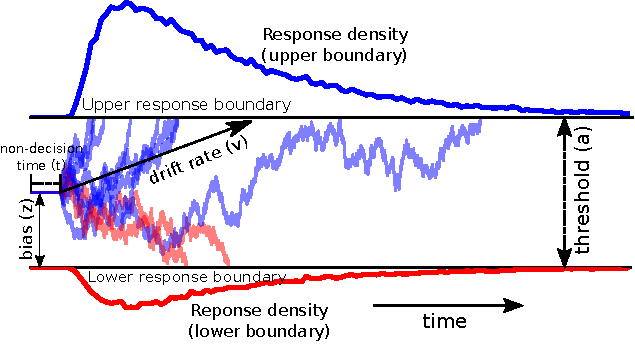
\includegraphics[scale=0.4]{DDM.pdf}
\caption{Trajectories of multiple drift-process (blue and red lines,
middle panel). Evidence is accumulated over time (x-axis) with
drift-rate v until one of two boundaries (separated by
threshold a) is crossed and a response is initiated. Upper (blue)
and lower (red) panels contain histograms over
boundary-crossing-times for two possible responses. The histogram
shapes match closely to that observed in reaction time
measurements of research participants.}\end{figure}

An analytic solution to the resulting probability distribution of
the termination times was provided by \citep{Feller68}:
\begin{gather}
\begin{split}f(t|v, a, z) = \frac{\pi}{a^2} \, \text{exp} \left( -vaz-\frac{v^2\,t}{2} \right) \times \sum_{k=1}^{\infty} k\, \text{exp} \left( -\frac{k^2\pi^2 t}{2a^2} \right) \text{sin}\left(k\pi z\right)\end{split}\notag
\end{gather}
Since the formula contains an infinite sum, HDDM uses an approximation
provided by \citep{NavarroFuss09}.

Later on, the DDM was extended to include additional noise parameters
capturing inter-trial variability in the drift-rate, the non-decision
time and the starting point in order to account for two phenomena
observed in decision making tasks, most notably cases where errors are
faster or slower than correct responses. Models that take this into
account are referred to as the full DDM
\citep{RatcliffRouder98}). HDDM uses analytic integration of the
likelihood function for variability in drift-rate and numerical
integration for variability in non-decision time and bias. More
information on the model specifics can be found in \citep{SoferWieckiFrank}.


\subsubsection{Linear Ballistic Accumulator}
\label{methods:linear-ballistic-accumulator}
The Linear Ballistic Accumulator (LBA) model belongs to the class of
race models \citep{BrownHeathcote08}). Instead of one drift process
and two boundaries, the LBA contains one drift process for each
possible response with a single boundary each. Thus, the LBA can model
decision making when more than two responses are possible. Moreover,
unlike the DDM, the LBA drift process has no intra-trial variance. RT
variability is obtained by including inter-trial variability in the
drift-rate and the starting point distribution. Note that the
simplifying assumption of a noiseless drift-process simplifies the
math significantly leading to a computationally more efficient
likelihood function for this model.

In a simulation study it was shown that the LBA and DDM lead to
similar results as to which parameters are affected by certain
manipulations \citep{DonkinBrownHeathcoteEtAl11}).
\begin{figure}[htbp]
\centering
\capstart

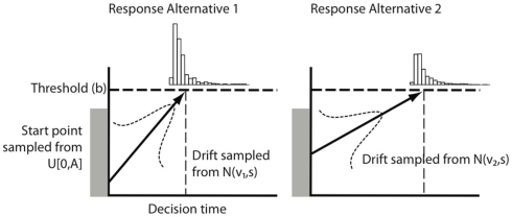
\includegraphics[scale=.4]{lba.png}
\caption{Two linear ballistic accumulators (left and right) with different
noiseless drifts (arrows) sampled from a normal distribution
initiated at different starting points sampled from a uniform
distribution. In this case, the accumulator for response
alternative 1 is more likely to reach the criterion first, and
therefore gets selected more often. Because of this race between
two accumulators towards a common threshold these model are called
race-models. Reproduced from \citep{DonkinBrownHeathcoteEtAl11}.}\end{figure}


\subsection{Hierarchical Bayesian Estimation}
\label{methods:hierarchical-bayesian-estimation}
Statistics and machine learning have developed efficient and versatile
Bayesian methods to solve various inference problems
\citep{Poirier06}. More recently, they have seen wider adoption in
applied fields such as genetics \citep{StephensBalding09} and
psychology \citep{ClemensDeSelenEtAl11}. One reason for this
Bayesian revolution is the ability to quantify the certainty one has
in a particular estimation. Moreover, hierarchical Bayesian models
provide an elegant solution to the problem of estimating parameters of
individual subjects and groups of subjects, as outlined above. Under the assumption that
participants within each group are similar to each other, but not
identical, a hierarchical model can be constructed where individual
parameter estimates are constrained by group-level distributions
\citep{NilssonRieskampWagenmakers11,ShiffrinLeeKim08}).

Bayesian methods require specification of a generative process in form
of a likelihood function that produced the observed data $x$
given some parameters $\theta$. By specifying our prior beliefs
(which can be informed or non-informed) we can use Bayes formula to
invert the generative model and make inference on the probability of
parameters $\theta$:
\phantomsection\label{methods:bayes}\begin{gather}
\begin{split}P(\theta|x) = \frac{P(x|\theta) \times P(\theta)}{P(x)}\end{split}\notag
\end{gather}
Where $P(x|\theta)$ is the likelihood of observing the data (in
this case choices and RTs) given each parameter value and
$P(\theta)$ is the prior probability of the parameters. In most
cases the computation of the denominator is quite complicated and
requires to compute an analytically intractable integral. Sampling
methods like Markov-Chain Monte Carlo (MCMC) \citep{GamermanLopes06}
circumvent this problem by providing a way to produce samples from the
posterior distribution. These methods have been used with great
success in many different scenarios \citep{GelmanCarlinSternEtAl03}
and will be discussed in more detail below.

As noted above, the Bayesian method lends itself naturally to a
hierarchical design. In such a design, parameters for one distribution
can themselves be drawn from a higher level distribution. This
hierarchical property has a particular benefit to cognitive modeling
where data is often scarce. We can construct a hierarchical model to
more adequately capture the likely similarity structure of our
data. As above, observed data points of each subject $x_{i,j}$
(where $i = 1, \dots, S_j$ data points per subject and $j
= 1, \dots, N$ for $N$ subjects) are distributed according to
some likelihood function $f | \theta$.  We now assume that
individual subject parameters $\theta_j$ are normally
distributed around a group mean $\mu$ with a specific group variance $\sigma$, resulting in
the following generative description:
\begin{gather}
\begin{split}
\theta_j &\sim \mathcal{N}(\mu, \sigma^2) \\
x_{i, j} &\sim f(\theta_j)\end{split}\notag
\end{gather}\begin{figure}[htbp]
\centering
\capstart

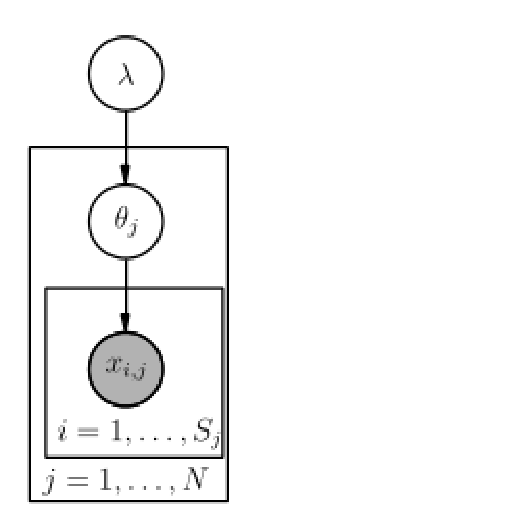
\includegraphics[scale=.6]{graphical_hierarchical.pdf}
\caption{Graphical notation of a hierarchical model. Circles represent
continuous random variables. Arrows connecting circles specify
conditional dependence between random variables. Shaded circles
represent observed data. Finally, plates around graphical nodes
mean that multiple identical, independent distributed random
variables exist.}\end{figure}


\subsection{Hierarchical Drift-Diffusion Models used in HDDM}
\label{methods:hierarchical-drift-diffusion-models-used-in-hddm}
HDDM includes several hierarchical Bayesian model formulations for the
DDM and LBA. For illustrative purposes we present the graphical model
depiction of a hierarchical DDM model with informative priors and
group only inter-trial variablity parameters. Note, however, that
there is also a model with non-informative priors.
\begin{figure}[htbp]
\centering
\capstart

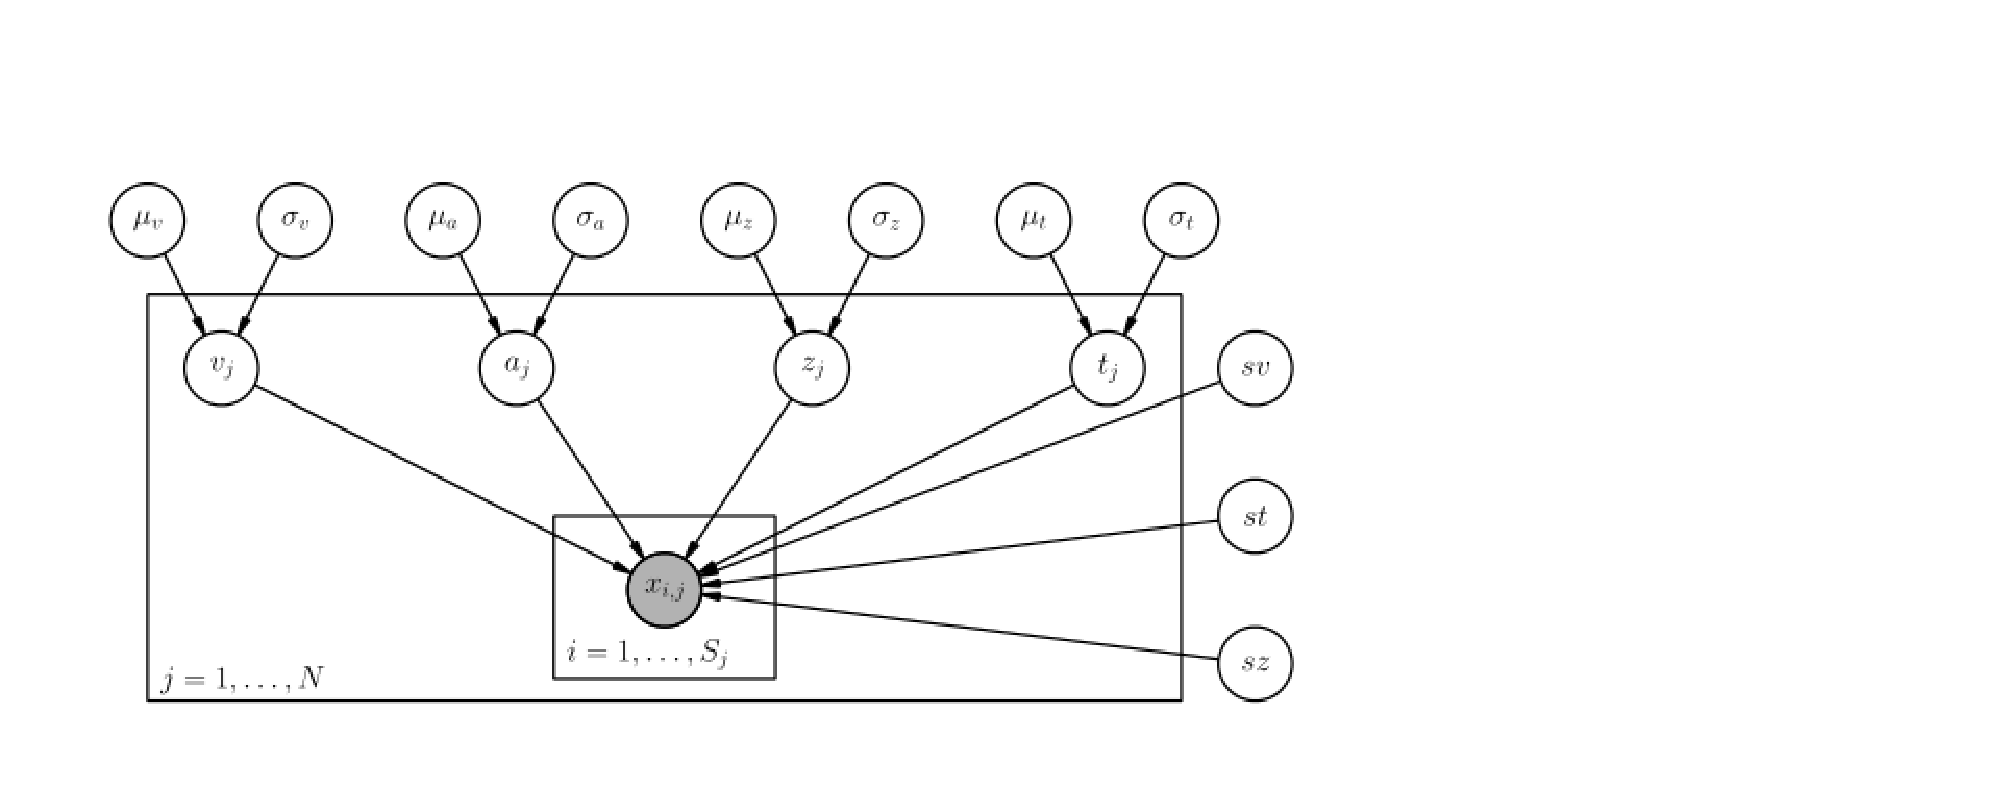
\includegraphics[scale=.5]{graphical_hddm.pdf}
\caption{Basic graphical hierarchical model implemented by HDDM for
estimation of the drift-diffusion model.}\end{figure}

Individual graphical nodes are distributed as follow:\\
\begin{center}
\begin{tabular}{l|l|l}
$\mu_{a} \sim \mathcal{G}(1.5, 0.75)$ & $\sigma_{a} \sim \mathcal{HN}(0.1)$ & $a_{j} \sim \mathcal{G}(\mu_{a}, \sigma_{a}^2)$ \\
$\mu_{v} \sim \mathcal{N}(2, 3)$ & $\sigma_{v} \sim \mathcal{HN}(2)$ & $v_{j} \sim \mathcal{N}(\mu_{v}, \sigma_{v}^2)$ \\

$\mu_{z} \sim \mathcal{N}(0.5, 0.5)$ & $\sigma_{z} \sim \mathcal{HN}(0.05)$ & $z_{j} \sim \text{invlogit}(\mathcal{N}(\mu_{z}, \sigma_{z}^2))$ \\

$\mu_{ter} \sim \mathcal{G}(0.4, 0.2)$ & $\sigma_{ter} \sim \mathcal{HN}(1)$ & $ter_{j} \sim \mathcal{N}(\mu_{ter}, \sigma_{ter}^2)$\\

$sv \sim \mathcal{HN}(2)$ & $ster \sim \mathcal{HN}(0.3)$ & $sz \sim \mathcal{B}(1, 3)$
\end{tabular}
\end{center}
and $x_{i, j} \sim F(a_{i}, z_{i}, v_{i}, ter_{i}, sv, ster, sz)$ where $x_{i, j}$ represents the observed data consisting of
reaction time and choice and $F$ represents the DDM likelihood
function as formulated by \citep{NavarroFuss09}. $\mathcal{N}$
represents a normal distribution parameterized by mean and standard
deviation, $\mathcal{HN}$ represents a half-normal parameterized
standard-deviation, $\mathcal{G}$ represents a Gamma
distribution parameterized by mean and rate, $\mathcal{B}$
represents a Beta distribution parameterized by $\alpha$ and
$\beta$. Note that in this model we do not attempt to estimate
individual parameters for inter-trial variabilities. The reason is
that the influence of these parameters onto the likelihood is often so
small that very large amounts of data would be required to make
meaningful inference at the individual level.

These priors are created to roughly match parameter values reported in
the literature and collected by \citep{MatzkeWagenmakers09}. In the
below figure we overlayed those empirical values with the prior
distribution used for each parameter.
\begin{figure}[htbp]
\centering

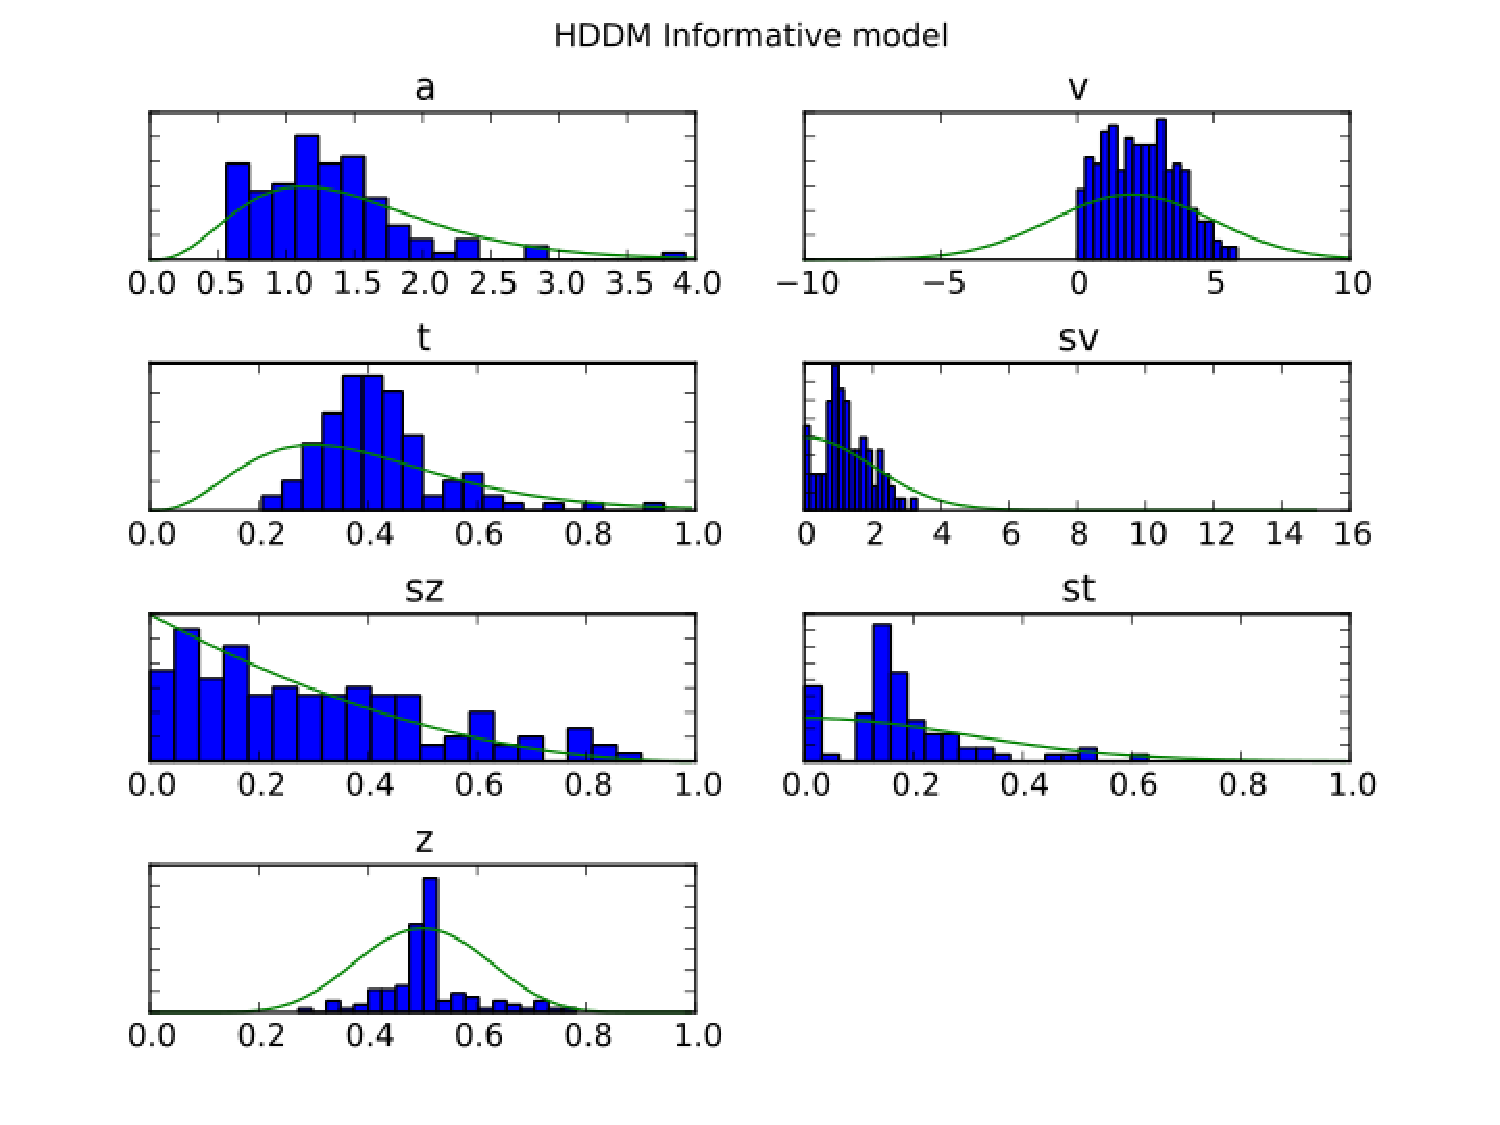
\includegraphics[scale=.5]{hddm_info_priors.pdf}
\end{figure}

HDDM then uses MCMC to estimate the joint posterior distribution of
all model parameters.

Note that the exact form of the model will be user-dependent; consider
as an example a model where separate drift-rates \emph{v} are estimated for
two conditions in an experiment: easy and hard. In this case, HDDM
will create a hierarchical model with group parameters
$\mu_{v_{\text{easy}}}$, $\sigma_{v_{\text{easy}}}$,
$\mu_{v_{\text{hard}}}$, $\sigma_{v_{\text{hard}}}$,and individual subject parameters $v_{j_{\text{easy}}}$, and $v_{j_{\text{hard}}}$.

\section{Results}
\label{demo:index-0}\label{demo:demo}\label{demo:chap-demo}\label{demo::doc}\label{demo:patsy}
In the following we will demonstrate how HDDM can be used to infer different components of the decision making process in a reward-based learning task. While demonstrating core features this is by no means a complete overview of all the functionality in HDDM. For more information, including on how to use HDDM as a command-line utility, online tutorial and a refernce manual see \href{http://ski.clps.brown.edu/hddm\_docs}{http://ski.clps.brown.edu/hddm\_docs}.

Python requires modules to be imported before they can be used.
\DUspan{keyword,namespace}{}\DUspan{name,namespace}{}\DUspan{keyword,namespace}{}\DUspan{name,namespace}{}\DUspan{keyword,namespace}{}\DUspan{name,namespace}{}
\begin{Verbatim}[commandchars=\\\{\}]
\PYG{k+kn}{import} \PYG{n+nn}{hddm}
\PYG{k+kn}{import} \PYG{n+nn}{matplotlib.pyplot} \PYG{k+kn}{as} \PYG{n+nn}{plt}
\end{Verbatim}

Matplotlib is Python module for generating graphics.

\subsection{Loading data}
\label{demo:loading-data}
It is recommended to store your trial-by-trial reaction time and choice data in a csv (comma-separated-value, see below for exact specifications) file. In this example we will be using data collected in a reward-based decision making experiment in our lab \citep{CavanaghWieckiCohenEtAl11}. In brief, at each trial subjects choose between two symbols. The trials were divided into win-win trials (WW), in which the two symbols were associated with high winning chances; lose-lose trials (LL), in which the symbols were associated with low winning chances, and win-lose trials (WL), which are the easiest because only one symbol was associated with high winning chances. Thus WW and LL decisions together comprise high conflict (HC) trials (although there are other differences between them, we don't focus on those here), whereas WL decisions are low conflict (LC).  The main hypothesis of the study was that high conflict trials induce an increase in the decision threshold, and that the mechanism for this threshold modulation depends on communication between mediofrontal cortex (which exhibits increased activity under conditions of choice uncertainty or conflict) and the subthalamic nucleus (STN) of the basal ganglia (which provides a temporary brake on response selection by increasing the decision threshold). The details of this mechanism are described in other modeling papers \citep[e.g.][]{RatcliffFrank12}. \citet{CavanaghWieckiCohenEtAl11} tested this theory by measuring EEG activity over mid-frontal cortex, focusing on the theta band, given prior associations with conflict, and testing whether trial-to-trial variations in frontal theta were related to adjustments in decision threshold during high conflict trials. They tested the STN component of the theory by administering the same experiment to patients who had deep brain stimulation (dbs) of the STN, which interferes with normal processing.

The first ten lines of the data file look as follows:
\DUspan{error}{}\DUspan{name}{}\DUspan{name}{}\DUspan{operator}{}\DUspan{name}{}
\begin{Verbatim}[commandchars=\\\{\}]
!head hddm\_demo.csv
\end{Verbatim}

\begin{Verbatim}[commandchars=\\\{\}]
\PYG{n}{subj\PYGZus{}idx}\PYG{p}{,}\PYG{n}{stim}\PYG{p}{,}\PYG{n}{rt}\PYG{p}{,}\PYG{n}{response}\PYG{p}{,}\PYG{n}{theta}\PYG{p}{,}\PYG{n}{dbs}\PYG{p}{,}\PYG{n}{conf}
\PYG{l+m+mi}{0}\PYG{p}{,}\PYG{n}{LL}\PYG{p}{,}\PYG{l+m+mf}{1.21}\PYG{p}{,}\PYG{l+m+mf}{1.0}\PYG{p}{,}\PYG{l+m+mf}{0.65627512226100004}\PYG{p}{,}\PYG{l+m+mi}{1}\PYG{p}{,}\PYG{n}{HC}
\PYG{l+m+mi}{0}\PYG{p}{,}\PYG{n}{WL}\PYG{p}{,}\PYG{l+m+mf}{1.6299999999999999}\PYG{p}{,}\PYG{l+m+mf}{1.0}\PYG{p}{,}\PYG{o}{\PYGZhy{}}\PYG{l+m+mf}{0.32788867166199998}\PYG{p}{,}\PYG{l+m+mi}{1}\PYG{p}{,}\PYG{n}{LC}
\PYG{l+m+mi}{0}\PYG{p}{,}\PYG{n}{WW}\PYG{p}{,}\PYG{l+m+mf}{1.03}\PYG{p}{,}\PYG{l+m+mf}{1.0}\PYG{p}{,}\PYG{o}{\PYGZhy{}}\PYG{l+m+mf}{0.480284512399}\PYG{p}{,}\PYG{l+m+mi}{1}\PYG{p}{,}\PYG{n}{HC}
\PYG{l+m+mi}{0}\PYG{p}{,}\PYG{n}{WL}\PYG{p}{,}\PYG{l+m+mf}{2.77}\PYG{p}{,}\PYG{l+m+mf}{1.0}\PYG{p}{,}\PYG{l+m+mf}{1.9274273452399999}\PYG{p}{,}\PYG{l+m+mi}{1}\PYG{p}{,}\PYG{n}{LC}
\PYG{l+m+mi}{0}\PYG{p}{,}\PYG{n}{WW}\PYG{p}{,}\PYG{l+m+mf}{1.1399999999999999}\PYG{p}{,}\PYG{l+m+mf}{0.0}\PYG{p}{,}\PYG{o}{\PYGZhy{}}\PYG{l+m+mf}{0.21323572605999999}\PYG{p}{,}\PYG{l+m+mi}{1}\PYG{p}{,}\PYG{n}{HC}
\PYG{l+m+mi}{0}\PYG{p}{,}\PYG{n}{WL}\PYG{p}{,}\PYG{l+m+mf}{1.1499999999999999}\PYG{p}{,}\PYG{l+m+mf}{1.0}\PYG{p}{,}\PYG{o}{\PYGZhy{}}\PYG{l+m+mf}{0.43620365940099998}\PYG{p}{,}\PYG{l+m+mi}{1}\PYG{p}{,}\PYG{n}{LC}
\PYG{l+m+mi}{0}\PYG{p}{,}\PYG{n}{LL}\PYG{p}{,}\PYG{l+m+mf}{2.0}\PYG{p}{,}\PYG{l+m+mf}{1.0}\PYG{p}{,}\PYG{o}{\PYGZhy{}}\PYG{l+m+mf}{0.27447891439400002}\PYG{p}{,}\PYG{l+m+mi}{1}\PYG{p}{,}\PYG{n}{HC}
\PYG{l+m+mi}{0}\PYG{p}{,}\PYG{n}{WL}\PYG{p}{,}\PYG{l+m+mf}{1.04}\PYG{p}{,}\PYG{l+m+mf}{0.0}\PYG{p}{,}\PYG{l+m+mf}{0.66695707371400004}\PYG{p}{,}\PYG{l+m+mi}{1}\PYG{p}{,}\PYG{n}{LC}
\PYG{l+m+mi}{0}\PYG{p}{,}\PYG{n}{WW}\PYG{p}{,}\PYG{l+m+mf}{0.85699999999999998}\PYG{p}{,}\PYG{l+m+mf}{1.0}\PYG{p}{,}\PYG{l+m+mf}{0.11861689909799999}\PYG{p}{,}\PYG{l+m+mi}{1}\PYG{p}{,}\PYG{n}{HC}
\end{Verbatim}

The \code{hddm.load\_csv()} function can then be used to load this file. \DUspan{name}{}\DUspan{operator}{}\DUspan{name}{}\DUspan{operator}{}\DUspan{name}{}\DUspan{punctuation}{}\DUspan{literal,string}{}\DUspan{punctuation}{}
\begin{Verbatim}[commandchars=\\\{\}]
\PYG{n}{data} \PYG{o}{=} \PYG{n}{hddm}\PYG{o}{.}\PYG{n}{load\PYGZus{}csv}\PYG{p}{(}\PYG{l+s}{\PYGZsq{}}\PYG{l+s}{hddm\PYGZus{}demo.csv}\PYG{l+s}{\PYGZsq{}}\PYG{p}{)}
\end{Verbatim}
\DUspan{name}{}\DUspan{operator}{}\DUspan{name}{}\DUspan{punctuation}{}\DUspan{literal,number,integer}{}\DUspan{punctuation}{}
\begin{Verbatim}[commandchars=\\\{\}]
\PYG{n}{data}\PYG{o}{.}\PYG{n}{head}\PYG{p}{(}\PYG{l+m+mi}{10}\PYG{p}{)}
\end{Verbatim}

\begin{Verbatim}[commandchars=\\\{\}]
   subj\_idx stim     rt  response     theta  dbs conf
0         0   LL  1.210         1  0.656275    1   HC
1         0   WL  1.630         1 -0.327889    1   LC
2         0   WW  1.030         1 -0.480285    1   HC
3         0   WL  2.770         1  1.927427    1   LC
4         0   WW  1.140         0 -0.213236    1   HC
5         0   WL  1.150         1 -0.436204    1   LC
6         0   LL  2.000         1 -0.274479    1   HC
7         0   WL  1.040         0  0.666957    1   LC
8         0   WW  0.857         1  0.118617    1   HC
9         0   WL  1.500         0  0.823626    1   LC
\end{Verbatim}

To provide a sense of what how RT data is normally distributed we next plot the histograms (we are using pandas' \code{groupby()} functionality to loop over the data corresponding to each invidual subject). Because there are two possible responses (here we are using accuracy coding where 1 means the more rewarding symbol was chosen, and 0 the less rewarding) we flip error RTs to be negative. \DUspan{name}{}\DUspan{operator}{}\DUspan{name}{}\DUspan{operator}{}\DUspan{name}{}\DUspan{operator}{}\DUspan{name}{}\DUspan{punctuation}{}\DUspan{name}{}\DUspan{punctuation}{}\DUspan{name}{}\DUspan{operator}{}\DUspan{name}{}\DUspan{operator}{}\DUspan{name}{}\DUspan{punctuation}{}\DUspan{name}{}\DUspan{operator}{}\DUspan{name}{}\DUspan{operator}{}\DUspan{name}{}\DUspan{punctuation}{}\DUspan{literal,number,integer}{}\DUspan{punctuation}{}\DUspan{name}{}\DUspan{operator}{}\DUspan{literal,string}{}\DUspan{punctuation}{}\DUspan{name}{}\DUspan{operator}{}\DUspan{literal,string}{}\DUspan{punctuation}{}\DUspan{name}{}\DUspan{operator}{}\DUspan{literal,string}{}\DUspan{punctuation}{}\DUspan{keyword}{}\DUspan{name}{}\DUspan{punctuation}{}\DUspan{name}{}\DUspan{operator,word}{}\DUspan{name}{}\DUspan{operator}{}\DUspan{name}{}\DUspan{punctuation}{}\DUspan{literal,string}{}\DUspan{punctuation}{}\DUspan{name}{}\DUspan{operator}{}\DUspan{name}{}\DUspan{punctuation}{}\DUspan{name}{}\DUspan{operator}{}\DUspan{name}{}\DUspan{punctuation}{}\DUspan{name}{}\DUspan{operator}{}\DUspan{literal,number,integer}{}\DUspan{punctuation}{}\DUspan{name}{}\DUspan{operator}{}\DUspan{literal,string}{}\DUspan{punctuation}{}
\begin{Verbatim}[commandchars=\\\{\}]
\PYG{n}{data} \PYG{o}{=} \PYG{n}{hddm}\PYG{o}{.}\PYG{n}{utils}\PYG{o}{.}\PYG{n}{flip\PYGZus{}errors}\PYG{p}{(}\PYG{n}{data}\PYG{p}{)}

\PYG{n}{fig} \PYG{o}{=} \PYG{n}{plt}\PYG{o}{.}\PYG{n}{figure}\PYG{p}{(}\PYG{p}{)}
\PYG{n}{ax} \PYG{o}{=} \PYG{n}{fig}\PYG{o}{.}\PYG{n}{add\PYGZus{}subplot}\PYG{p}{(}\PYG{l+m+mi}{111}\PYG{p}{,} \PYG{n}{xlabel}\PYG{o}{=}\PYG{l+s}{\PYGZsq{}}\PYG{l+s}{RT}\PYG{l+s}{\PYGZsq{}}\PYG{p}{,} \PYG{n}{ylabel}\PYG{o}{=}\PYG{l+s}{\PYGZsq{}}\PYG{l+s}{count}\PYG{l+s}{\PYGZsq{}}\PYG{p}{,} \PYG{n}{title}\PYG{o}{=}\PYG{l+s}{\PYGZsq{}}\PYG{l+s}{RT distributions}\PYG{l+s}{\PYGZsq{}}\PYG{p}{)}
\PYG{k}{for} \PYG{n}{i}\PYG{p}{,} \PYG{n}{subj\PYGZus{}data} \PYG{o+ow}{in} \PYG{n}{data}\PYG{o}{.}\PYG{n}{groupby}\PYG{p}{(}\PYG{l+s}{\PYGZsq{}}\PYG{l+s}{subj\PYGZus{}idx}\PYG{l+s}{\PYGZsq{}}\PYG{p}{)}\PYG{p}{:}
    \PYG{n}{ax}\PYG{o}{.}\PYG{n}{hist}\PYG{p}{(}\PYG{n}{subj\PYGZus{}data}\PYG{o}{.}\PYG{n}{rt}\PYG{p}{,} \PYG{n}{bins}\PYG{o}{=}\PYG{l+m+mi}{20}\PYG{p}{,} \PYG{n}{histtype}\PYG{o}{=}\PYG{l+s}{\PYGZsq{}}\PYG{l+s}{step}\PYG{l+s}{\PYGZsq{}}\PYG{p}{)}
\end{Verbatim}

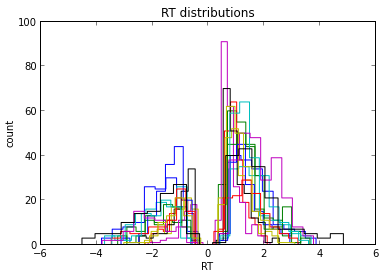
\includegraphics{hddm_demo_fig_00.png}


\subsection{Fitting a hierarchical model}
\label{demo:fitting-a-hierarchical-model}
The previous figure shows that while each individual's RT histogram is different, there is also a lot of similarity. Hierarchical Bayesian modeling allows us to exploit this similarity. The \code{HDDM} class constructs such a hierarchical DDM. The {HDDM.sample()} method then performs Bayesian inference by drawing posterior samples using the MCMC algorithm.
\DUspan{comment}{}\DUspan{comment}{}\DUspan{name}{}\DUspan{operator}{}\DUspan{name}{}\DUspan{operator}{}\DUspan{name}{}\DUspan{punctuation}{}\DUspan{name}{}\DUspan{punctuation}{}\DUspan{comment}{}\DUspan{name}{}\DUspan{operator}{}\DUspan{name}{}\DUspan{punctuation}{}\DUspan{comment}{}\DUspan{name}{}\DUspan{operator}{}\DUspan{name}{}\DUspan{punctuation}{}\DUspan{literal,number,integer}{}\DUspan{punctuation}{}\DUspan{name}{}\DUspan{operator}{}\DUspan{literal,number,integer}{}\DUspan{punctuation}{}
\begin{Verbatim}[commandchars=\\\{\}]
\PYG{c}{\PYGZsh{} Instantiate model object passing it our data (no need to call flip\PYGZus{}errors() before passing it).}
\PYG{c}{\PYGZsh{} This will tailor an individual hierarchical DDM around the dataset.}
\PYG{n}{m} \PYG{o}{=} \PYG{n}{hddm}\PYG{o}{.}\PYG{n}{HDDM}\PYG{p}{(}\PYG{n}{data}\PYG{p}{)}
\PYG{c}{\PYGZsh{} find a good starting point which helps with the convergence.}
\PYG{n}{m}\PYG{o}{.}\PYG{n}{find\PYGZus{}starting\PYGZus{}values}\PYG{p}{(}\PYG{p}{)}
\PYG{c}{\PYGZsh{} start drawing 2000 samples and discarding 20 as burn\PYGZhy{}in}
\PYG{n}{m}\PYG{o}{.}\PYG{n}{sample}\PYG{p}{(}\PYG{l+m+mi}{2000}\PYG{p}{,} \PYG{n}{burn}\PYG{o}{=}\PYG{l+m+mi}{20}\PYG{p}{)}
\end{Verbatim}

It is critical to assess the statistics of our estimated model. The
\code{HDDM.print\_stats()} method outputs a table of summary statistics for each parameters' posterior (note that the output is abridged due to its length).
\DUspan{name}{}\DUspan{operator}{}\DUspan{name}{}\DUspan{operator}{}\DUspan{name}{}\DUspan{punctuation}{}\DUspan{name}{}\DUspan{punctuation}{}\DUspan{name}{}\DUspan{operator}{}\DUspan{name}{}\DUspan{operator}{}\DUspan{name}{}\DUspan{punctuation}{}\DUspan{literal,string}{}\DUspan{punctuation}{}\DUspan{literal,string}{}\DUspan{punctuation}{}\DUspan{literal,string}{}\DUspan{punctuation}{}\DUspan{literal,string}{}\DUspan{punctuation}{}
\begin{Verbatim}[commandchars=\\\{\}]
\PYG{n}{stats} \PYG{o}{=} \PYG{n}{m}\PYG{o}{.}\PYG{n}{gen\PYGZus{}stats}\PYG{p}{(}\PYG{p}{)}
\PYG{n}{stats}\PYG{p}{[}\PYG{n}{stats}\PYG{o}{.}\PYG{n}{index}\PYG{o}{.}\PYG{n}{isin}\PYG{p}{(}\PYG{p}{[}\PYG{l+s}{\PYGZsq{}}\PYG{l+s}{a}\PYG{l+s}{\PYGZsq{}}\PYG{p}{,} \PYG{l+s}{\PYGZsq{}}\PYG{l+s}{a\PYGZus{}var}\PYG{l+s}{\PYGZsq{}}\PYG{p}{,} \PYG{l+s}{\PYGZsq{}}\PYG{l+s}{a\PYGZus{}subj.0}\PYG{l+s}{\PYGZsq{}}\PYG{p}{,} \PYG{l+s}{\PYGZsq{}}\PYG{l+s}{a\PYGZus{}subj.1}\PYG{l+s}{\PYGZsq{}}\PYG{p}{]}\PYG{p}{)}\PYG{p}{]}
\end{Verbatim}

\begin{Verbatim}[commandchars=\\\{\}]
              mean       std      2.5q       25q       50q       75q 97.5q

a         2.058015  0.102570  1.862412  1.988854  2.055198  2.123046 2.261410
a\_var     0.379303  0.089571  0.244837  0.316507  0.367191  0.426531 0.591643
a\_subj.0  2.384066  0.059244  2.274352  2.340795  2.384700  2.423012 2.500647
a\_subj.1  2.127582  0.061901  2.003605  2.086776  2.126963  2.166261 2.254350

            mc err
a         0.002539
a\_var     0.002973
a\_subj.0  0.001727
a\_subj.1  0.002113
\end{Verbatim}

The output contains various summary statistics describing the posterior of each parameter: group mean parameter for
threshold \code{a}, group variability \code{a\_var} and individual subject parameters \code{a\_subj.0}. Other parameters are not shown here but were still estimated.

The inference algorithm, MCMC, requires the chains of the model to have properly converged. While there is no way to guarantee convergence for a finite set of samples in MCMC, there are many heuristics that allow identification of problems of convergence. One main analysis to investigate is the trace, the autocorrelation, and the marginal posterior. These can be plotted using the \code{HDDM.plot\_posteriors()} method. For the sake of brevity we only plot one here. In practice, however, one should examine all of them. \DUspan{name}{}\DUspan{operator}{}\DUspan{name}{}\DUspan{punctuation}{}\DUspan{literal,string}{}\DUspan{punctuation}{}\DUspan{literal,string}{}\DUspan{punctuation}{}\DUspan{literal,string}{}\DUspan{punctuation}{}\DUspan{literal,string}{}\DUspan{punctuation}{}
\begin{Verbatim}[commandchars=\\\{\}]
\PYG{n}{m}\PYG{o}{.}\PYG{n}{plot\PYGZus{}posteriors}\PYG{p}{(}\PYG{p}{[}\PYG{l+s}{\PYGZsq{}}\PYG{l+s}{a}\PYG{l+s}{\PYGZsq{}}{]}\PYG{p}{)}
\end{Verbatim}

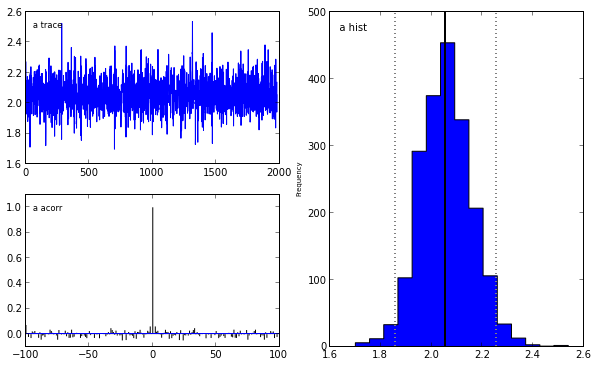
\includegraphics[scale=.5]{hddm_demo_fig_01.png}

Problematic patterns in the trace would be drifts or large jumps which are absent here. The autocorrelation should also not be exceedingly high as is here the case.

While these above steps increase confidence in whether the samples stem from the true posterior, these analyses do not convey how well the model actually fits the data. A posterior predictive check is commonly used to assess absolute model fit. A visual depiction of this can be created by calling the \code{HDDM.plot\_posterior\_predictive()} method. This will create a plot for each individual subject RT distribution in red on top of the predictive likelihood in blue. Intuitively, the two lines should match closely if the model provides a good fit to the data. \DUspan{name}{}\DUspan{operator}{}\DUspan{name}{}\DUspan{punctuation}{}\DUspan{name}{}\DUspan{operator}{}\DUspan{punctuation}{}\DUspan{literal,number,integer}{}\DUspan{punctuation}{}\DUspan{literal,number,integer}{}\DUspan{punctuation}{}
\begin{Verbatim}[commandchars=\\\{\}]
\PYG{n}{m}\PYG{o}{.}\PYG{n}{plot\PYGZus{}posterior\PYGZus{}predictive}\PYG{p}{(}\PYG{n}{figsize}\PYG{o}{=}\PYG{p}{(}\PYG{l+m+mi}{14}\PYG{p}{,} \PYG{l+m+mi}{10}\PYG{p}{)}\PYG{p}{)}
\end{Verbatim}

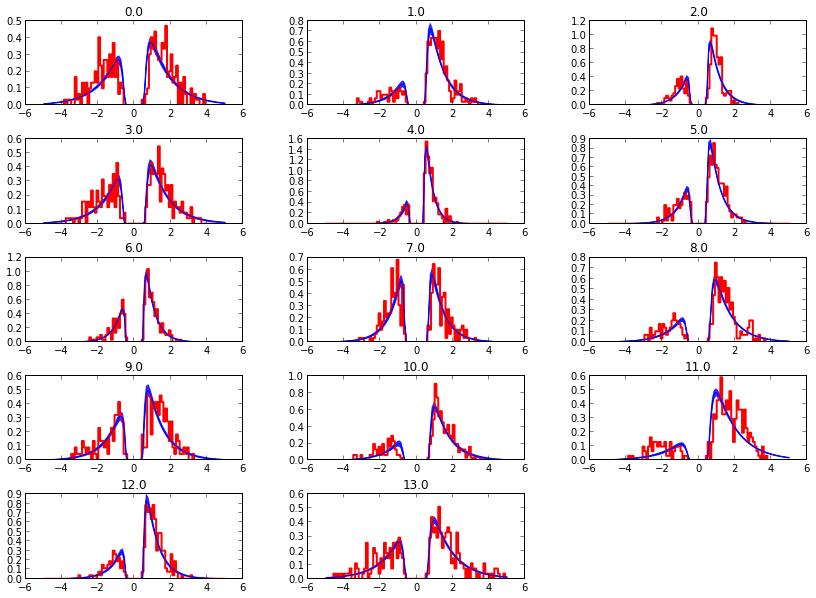
\includegraphics{hddm_demo_fig_05.png}

While the fit looks appropriate visually, we also have prior knowledge about the structure of the data as a result of our experimental procedure. For example, we would expect that because LL and WW trials are harder than WL trials, drift rate would be higher in WL, which has lower uncertainty about the correct choice. (One could also develop a posterior predictive check statistic that would evaluate whether accuracy and mean RT are different in the different conditions. Since the parameters of the model were estimated to be the same across conditions, the posterior predictive distributions for these conditions would not look different from each other, whereas those in the data do. A formal posterior predictive check would thus show that the data violates the simple assumptions of the model. This is not evident above because we simply plotted the distributions collapsed across conditions).

To test this hypothesis we create a new model which estimates separate drift-rate \code{v} for those different conditions by using the \code{depends\_on} keyword argument to \code{HDDM}. This argument expects a Python \code{dict} which maps the parameter to be split to the column name containing the conditions we want to split by. \DUspan{name}{}\DUspan{operator}{}\DUspan{name}{}\DUspan{operator}{}\DUspan{name}{}\DUspan{punctuation}{}\DUspan{name}{}\DUspan{punctuation}{}\DUspan{name}{}\DUspan{operator}{}\DUspan{punctuation}{}\DUspan{literal,string}{}\DUspan{punctuation}{}\DUspan{literal,string}{}\DUspan{punctuation}{}\DUspan{name}{}\DUspan{operator}{}\DUspan{name}{}\DUspan{punctuation}{}\DUspan{name}{}\DUspan{operator}{}\DUspan{name}{}\DUspan{punctuation}{}\DUspan{literal,number,integer}{}\DUspan{punctuation}{}\DUspan{name}{}\DUspan{operator}{}\DUspan{literal,number,integer}{}\DUspan{punctuation}{}
\begin{Verbatim}[commandchars=\\\{\}]
\PYG{n}{m\PYGZus{}stim} \PYG{o}{=} \PYG{n}{hddm}\PYG{o}{.}\PYG{n}{HDDM}\PYG{p}{(}\PYG{n}{data}\PYG{p}{,} \PYG{n}{depends\PYGZus{}on}\PYG{o}{=}\PYG{p}{\PYGZob{}}\PYG{l+s}{\PYGZsq{}}\PYG{l+s}{v}\PYG{l+s}{\PYGZsq{}}\PYG{p}{:} \PYG{l+s}{\PYGZsq{}}\PYG{l+s}{stim}\PYG{l+s}{\PYGZsq{}}\PYG{p}{\PYGZcb{}}\PYG{p}{)}
\PYG{n}{m\PYGZus{}stim}\PYG{o}{.}\PYG{n}{find\PYGZus{}starting\PYGZus{}values}\PYG{p}{(}\PYG{p}{)}
\PYG{n}{m\PYGZus{}stim}\PYG{o}{.}\PYG{n}{sample}\PYG{p}{(}\PYG{l+m+mi}{2000}\PYG{p}{,} \PYG{n}{burn}\PYG{o}{=}\PYG{l+m+mi}{20}\PYG{p}{)}
\end{Verbatim}

By examining the posterior for the different drift-rate conditions we can conclude that the WL condition drift-rate is substantially greater than that for the other two conditions, which are fairly similar to each other\footnote{While it would be easy to provide syntacic sugar for the below expression there are many cases where you want access to the underlying distributions. These are stored inside of \code{nodes\_db} which is a pandas \code{DataFrame} containing information about each distribution. Here we retrieve the actual node objects containing the trace from the \code{node} column.}. \DUspan{name}{}\DUspan{punctuation}{}\DUspan{name}{}\DUspan{punctuation}{}\DUspan{name}{}\DUspan{operator}{}\DUspan{name}{}\DUspan{operator}{}\DUspan{name}{}\DUspan{operator}{}\DUspan{name}{}\DUspan{punctuation}{}\DUspan{literal,string}{}\DUspan{punctuation}{}\DUspan{literal,string}{}\DUspan{punctuation}{}\DUspan{literal,string}{}\DUspan{punctuation}{}\DUspan{name}{}\DUspan{operator}{}\DUspan{name}{}\DUspan{operator}{}\DUspan{name}{}\DUspan{punctuation}{}\DUspan{name}{}\DUspan{punctuation}{}\DUspan{name}{}\DUspan{punctuation}{}\DUspan{name}{}\DUspan{punctuation}{}
\begin{Verbatim}[commandchars=\\\{\}]
\PYG{n}{v\PYGZus{}WW}\PYG{p}{,} \PYG{n}{v\PYGZus{}LL}\PYG{p}{,} \PYG{n}{v\PYGZus{}WL} \PYG{o}{=} \PYG{n}{m\PYGZus{}stim}\PYG{o}{.}\PYG{n}{nodes\PYGZus{}db}\PYG{o}{.}\PYG{n}{node}\PYG{p}{[}\PYG{p}{[}\PYG{l+s}{\PYGZsq{}}\PYG{l+s}{v(WW)}\PYG{l+s}{\PYGZsq{}}\PYG{p}{,} \PYG{l+s}{\PYGZsq{}}\PYG{l+s}{v(LL)}\PYG{l+s}{\PYGZsq{}}\PYG{p}{,} \PYG{l+s}{\PYGZsq{}}\PYG{l+s}{v(WL)}\PYG{l+s}{\PYGZsq{}}\PYG{p}{]}\PYG{p}{]}
\PYG{n}{hddm}\PYG{o}{.}\PYG{n}{analyze}\PYG{o}{.}\PYG{n}{plot\PYGZus{}posterior\PYGZus{}nodes}\PYG{p}{(}\PYG{p}{[}\PYG{n}{v\PYGZus{}WW}\PYG{p}{,} \PYG{n}{v\PYGZus{}LL}\PYG{p}{,} \PYG{n}{v\PYGZus{}WL}\PYG{p}{]}\PYG{p}{)}
\end{Verbatim}

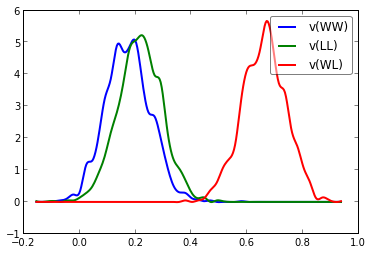
\includegraphics[scale=.7]{hddm_demo_fig_06.png}

One benefit of estimating the model in a Bayesian framework is that we can do significance testing directly on the posterior rather than relying on frequentist statistics (See Kruschke's book for many examples of the advantages of this approach). For example, we might be interested in whether the drift-rate for WW is larger than that for LL, or whether drift-rate for LL is larger than WL. The below code computes the proportion of the posteriors in which the drift rate for one condition is greater than the other. It can be seen that the posteriors for LL do not overlap at all for WL, and thus the probability that LL is greater than WL should be near zero. \DUspan{keyword}{}\DUspan{literal,string}{}\DUspan{punctuation}{}\DUspan{punctuation}{}\DUspan{name}{}\DUspan{operator}{}\DUspan{name}{}\DUspan{punctuation}{}\DUspan{operator}{}\DUspan{name}{}\DUspan{operator}{}\DUspan{name}{}\DUspan{punctuation}{}\DUspan{operator}{}\DUspan{name}{}\DUspan{punctuation}{}\DUspan{keyword}{}\DUspan{literal,string}{}\DUspan{punctuation}{}\DUspan{punctuation}{}\DUspan{name}{}\DUspan{operator}{}\DUspan{name}{}\DUspan{punctuation}{}\DUspan{operator}{}\DUspan{name}{}\DUspan{operator}{}\DUspan{name}{}\DUspan{punctuation}{}\DUspan{operator}{}\DUspan{name}{}\DUspan{punctuation}{}
\begin{Verbatim}[commandchars=\\\{\}]
\PYG{k}{print} \PYG{l+s}{\PYGZdq{}}\PYG{l+s}{P(WW \PYGZgt{} LL) = }\PYG{l+s}{\PYGZdq{}}\PYG{p}{,} \PYG{p}{(}\PYG{n}{v\PYGZus{}WW}\PYG{o}{.}\PYG{n}{trace}\PYG{p}{(}\PYG{p}{)} \PYG{o}{\PYGZgt{}} \PYG{n}{v\PYGZus{}LL}\PYG{o}{.}\PYG{n}{trace}\PYG{p}{(}\PYG{p}{)}\PYG{p}{)}\PYG{o}{.}\PYG{n}{mean}\PYG{p}{(}\PYG{p}{)}
\PYG{k}{print} \PYG{l+s}{\PYGZdq{}}\PYG{l+s}{P(LL \PYGZgt{} WL) = }\PYG{l+s}{\PYGZdq{}}\PYG{p}{,} \PYG{p}{(}\PYG{n}{v\PYGZus{}LL}\PYG{o}{.}\PYG{n}{trace}\PYG{p}{(}\PYG{p}{)} \PYG{o}{\PYGZgt{}} \PYG{n}{v\PYGZus{}WL}\PYG{o}{.}\PYG{n}{trace}\PYG{p}{(}\PYG{p}{)}\PYG{p}{)}\PYG{o}{.}\PYG{n}{mean}\PYG{p}{(}\PYG{p}{)}
\end{Verbatim}

\begin{Verbatim}[commandchars=\\\{\}]
\PYG{n}{P}\PYG{p}{(}\PYG{n}{WW} \PYG{o}{\PYGZgt{}} \PYG{n}{LL}\PYG{p}{)} \PYG{o}{=}  \PYG{l+m+mf}{0.34696969697}
\PYG{n}{P}\PYG{p}{(}\PYG{n}{LL} \PYG{o}{\PYGZgt{}} \PYG{n}{WL}\PYG{p}{)} \PYG{o}{=}  \PYG{l+m+mf}{0.0}
\end{Verbatim}

In addition to computing the overlap of the posterior distributions we can compare two models using the deviance information criterion (DIC; lower is better). Note that the DIC measures the fit of the model to the data, penalizing for complexity in the addition of degrees of freedom (the model with three drift rates has more dF than the model with one). The DIC is known to be somewhat biased in selecting the model with greater complexity, although alternative forms exist \citep[see][]{Plummer08}. Nevertheless, DIC can be a useful metric with this caveat in mind. \DUspan{keyword}{}\DUspan{literal,string}{}\DUspan{literal,string,interpol}{}\DUspan{literal,string}{}\DUspan{operator}{}\DUspan{name}{}\DUspan{operator}{}\DUspan{name}{}\DUspan{keyword}{}\DUspan{literal,string}{}\DUspan{literal,string,interpol}{}\DUspan{literal,string}{}\DUspan{operator}{}\DUspan{name}{}\DUspan{operator}{}\DUspan{name}{}
\begin{Verbatim}[commandchars=\\\{\}]
\PYG{k}{print} \PYG{l+s}{\PYGZdq{}}\PYG{l+s}{Lumped model DIC: }\PYG{l+s+si}{\PYGZpc{}f}\PYG{l+s}{\PYGZdq{}} \PYG{o}{\PYGZpc{}} \PYG{n}{m}\PYG{o}{.}\PYG{n}{dic}
\PYG{k}{print} \PYG{l+s}{\PYGZdq{}}\PYG{l+s}{Stimulus model DIC: }\PYG{l+s+si}{\PYGZpc{}f}\PYG{l+s}{\PYGZdq{}} \PYG{o}{\PYGZpc{}} \PYG{n}{m\PYGZus{}stim}\PYG{o}{.}\PYG{n}{dic}
\end{Verbatim}

\begin{Verbatim}[commandchars=\\\{\}]
Lumped model DIC: 10960.570932
Stimulus model DIC: 10775.615192
\end{Verbatim}


\subsection{Within-subject effects}
\label{demo:within-subject-effects}
Note that while the \code{m\_stim} model we created above estimates different drift-rates \code{v} for each subject, it implicitly assumes that the different conditions are completely independent of each other, because each drift rate was sampled from a separate group prior. However, there may be individual differences in overall performance, and if so it is reasonable to assume that someone who would be better at \code{WL} would also be better at \code{LL}. To model this intuition we can use a within-subject model where an intercept is used to capture overall performance in the `WL' condition as a baseline, and then the other \code{LL} and \code{WW} conditions are expressed relative to \code{WL}. (Perhaps every subject has a higher drift in WL than LL but there is huge variance in their overall drift rates. In this scenario, the earlier model would not have the power to detect the effect of condition on this within subject effect, because there would be large posterior variance in all of the drift rates, which would then overlap with each other.  In contrast, the within-subject model would estimate large variance in the intercept but still allow the model to infer a non-zero effect of condition with high precision).

The \code{HDDMRegressor} class supports modeling within-subject effects. In addition to the data, this class's constructor expects a linear model descriptor string. This descriptor contains the \code{outcome} variable that should be replaced with the output of the linear model -- in this case \code{v}. The \code{C()} specifies that the \code{stim} column contains categorical data. The \code{Treatment} argument encodes which condition should be used as the intercept. The two other conditions -- \code{LL} and \code{WW} -- will then be expressed \textit{relative} to \code{WL}. Internally, \code{HDDMRegressor} uses \code{Patsy} to construct a design matrix from the linear model descriptor, see \href{https://patsy.readthedocs.org/en/latest/}{https://patsy.readthedocs.org/en/latest/} for more details. \DUspan{name}{}\DUspan{operator}{}\DUspan{name}{}\DUspan{operator}{}\DUspan{name}{}\DUspan{punctuation}{}\DUspan{name}{}\DUspan{punctuation}{}\DUspan{literal,string}{}\DUspan{punctuation}{}
\begin{Verbatim}[commandchars=\\\{\}]
\PYG{n}{m\PYGZus{}within\PYGZus{}subj} \PYG{o}{=} \PYG{n}{hddm}\PYG{o}{.}\PYG{n}{HDDMRegressor}\PYG{p}{(}\PYG{n}{data}\PYG{p}{,} \PYG{l+s}{\PYGZdq{}}\PYG{l+s}{v \PYGZti{} C(stim, Treatment(}\PYG{l+s}{\PYGZsq{}}\PYG{l+s}{WL}\PYG{l+s}{\PYGZsq{}}\PYG{l+s}{))}\PYG{l+s}{\PYGZdq{}}\PYG{p}{)}
\end{Verbatim}

Which outputs the newly created covariates which will be used in the regression:
\begin{Verbatim}[commandchars=\\\{\}]
Adding these covariates:
['v\_Intercept', "v\_C(stim, Treatment('WL'))[T.LL]", "v\_C(stim, Treatment('WL'))[T.WW]"]
\end{Verbatim}

To estimate the model we again have to draw samples from the posterior:
\DUspan{name}{}\DUspan{operator}{}\DUspan{name}{}\DUspan{punctuation}{}\DUspan{literal,number,integer}{}\DUspan{punctuation}{}\DUspan{name}{}\DUspan{operator}{}\DUspan{literal,number,integer}{}\DUspan{punctuation}{}
\begin{Verbatim}[commandchars=\\\{\}]
\PYG{n}{m\PYGZus{}within\PYGZus{}subj}\PYG{o}{.}\PYG{n}{sample}\PYG{p}{(}\PYG{l+m+mi}{5000}\PYG{p}{,} \PYG{n}{burn}\PYG{o}{=}\PYG{l+m+mi}{200}\PYG{p}{)}
\end{Verbatim}
\DUspan{name}{}\DUspan{punctuation}{}\DUspan{name}{}\DUspan{punctuation}{}\DUspan{name}{}\DUspan{operator}{}\DUspan{name}{}\DUspan{operator}{}\DUspan{name}{}\DUspan{operator}{}\DUspan{name}{}\DUspan{punctuation}{}\DUspan{literal,string}{}\DUspan{punctuation}{}\DUspan{literal,string}{}\DUspan{punctuation}{}\DUspan{literal,string}{}\DUspan{punctuation}{}\DUspan{name}{}\DUspan{operator}{}\DUspan{name}{}\DUspan{operator}{}\DUspan{name}{}\DUspan{punctuation}{}\DUspan{name}{}\DUspan{punctuation}{}\DUspan{name}{}\DUspan{punctuation}{}\DUspan{name}{}\DUspan{punctuation}{}

To examine the marginal posteriors of our individual regressors we can again plot them:
\begin{Verbatim}[commandchars=\\\{\}]
\PYG{n}{v\PYGZus{}WL}\PYG{p}{,} \PYG{n}{v\PYGZus{}LL}\PYG{p}{,} \PYG{n}{v\PYGZus{}WW} \PYG{o}{=} \PYG{n}{m\PYGZus{}within\PYGZus{}subj}\PYG{o}{.}\PYG{n}{nodes\PYGZus{}db}\PYG{o}{.}\PYG{n}{node}\PYG{p}{[}\PYG{p}{[}\PYG{l+s}{\PYGZdq{}}\PYG{l+s}{v\PYGZus{}Intercept}\PYG{l+s}{\PYGZdq{}}\PYG{p}{,}
                                                \PYG{l+s}{\PYGZdq{}}\PYG{l+s}{v\PYGZus{}C(stim, Treatment(}\PYG{l+s}{\PYGZsq{}}\PYG{l+s}{WL}\PYG{l+s}{\PYGZsq{}}\PYG{l+s}{))[T.LL]}\PYG{l+s}{\PYGZdq{}}\PYG{p}{,}
                                                \PYG{l+s}{\PYGZdq{}}\PYG{l+s}{v\PYGZus{}C(stim, Treatment(}\PYG{l+s}{\PYGZsq{}}\PYG{l+s}{WL}\PYG{l+s}{\PYGZsq{}}\PYG{l+s}{))[T.WW]}\PYG{l+s}{\PYGZdq{}}\PYG{p}{]}\PYG{p}{]}
\PYG{n}{kabuki}\PYG{o}{.}\PYG{n}{analyze}\PYG{o}{.}\PYG{n}{plot\PYGZus{}posterior\PYGZus{}nodes}\PYG{p}{(}\PYG{p}{[}\PYG{n}{v\PYGZus{}WL}\PYG{p}{,} \PYG{n}{v\PYGZus{}LL}\PYG{p}{,} \PYG{n}{v\PYGZus{}WW}\PYG{p}{]}\PYG{p}{)}
\end{Verbatim}

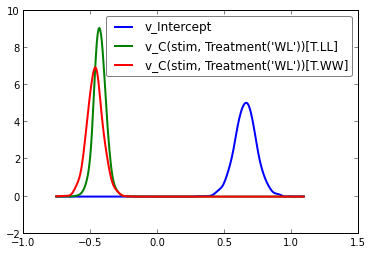
\includegraphics[scale=.7]{hddm_demo_fig_07.png}

Note that in the above plot \code{LL} and \code{WW} are expressed relative to the \code{WL} condition (i.e. \code{v\_Intercept}). Thus, while the overall drift rate intercept, here applying to the \code{WL} condition, is positive (mode value roughly 0.7), the relative within subject effects of condition (\code{WW} and \code{LL}) are negative and do not overlap with zero suggesting a significant effect of this condition on drift-rate.

\subsection{Fitting regression models}
\label{demo:fitting-regression-models}
As mentioned above, cognitive neuroscience has embraced the DDM as it enables to link psychological processes to cognitive brain measures. The \citet{CavanaghWieckiCohenEtAl11} study is a great example of this. EEG recordings provided a trial-ty-trial measure of brain activity (frontal theta), and it was found that this activity correlated with increases in decision threshold in high conflict trials. Note that the data set and results exhibit more features than we consider here for the time being (specifically the manipulation of deep brain stimulation), but for illustrative purposes, we replicate here that main theta-threshold relationship in a model restricted to participants without brain stimulation. For more information, see \href{http://ski.clps.brown.edu/papers/Cavanagh\_DBSEEG.pdf}{http://ski.clps.brown.edu/papers/Cavanagh\_DBSEEG.pdf} \DUspan{name}{}\DUspan{operator}{}\DUspan{name}{}\DUspan{operator}{}\DUspan{name}{}\DUspan{punctuation}{}\DUspan{name}{}\DUspan{punctuation}{}\DUspan{name}{}\DUspan{operator}{}\DUspan{name}{}\DUspan{operator}{}\DUspan{literal,number,integer}{}\DUspan{punctuation}{}\DUspan{literal,string}{}\DUspan{punctuation}{}\DUspan{name}{}\DUspan{operator}{}\DUspan{punctuation}{}\DUspan{literal,string}{}\DUspan{punctuation}{}\DUspan{literal,string}{}\DUspan{punctuation}{}\DUspan{name}{}\DUspan{operator}{}\DUspan{name,builtin,pseudo}{}\DUspan{punctuation}{}
\begin{Verbatim}[commandchars=\\\{\}]
\PYG{n}{m\PYGZus{}reg} \PYG{o}{=} \PYG{n}{hddm}\PYG{o}{.}\PYG{n}{HDDMRegressor}\PYG{p}{(}\PYG{n}{data}\PYG{p}{[}\PYG{n}{data}\PYG{o}{.}\PYG{n}{dbs} \PYG{o}{==} \PYG{l+m+mi}{0}\PYG{p}{]}\PYG{p}{,}
                           \PYG{l+s}{\PYGZdq{}}\PYG{l+s}{a \PYGZti{} theta:C(conf, Treatment(}\PYG{l+s}{\PYGZsq{}}\PYG{l+s}{LC}\PYG{l+s}{\PYGZsq{}}\PYG{l+s}{))}\PYG{l+s}{\PYGZdq{}}\PYG{p}{,}
                           \PYG{n}{depends\PYGZus{}on}\PYG{o}{=}\PYG{p}{\PYGZob{}}\PYG{l+s}{\PYGZsq{}}\PYG{l+s}{v}\PYG{l+s}{\PYGZsq{}}\PYG{p}{:} \PYG{l+s}{\PYGZsq{}}\PYG{l+s}{stim}\PYG{l+s}{\PYGZsq{}}\PYG{p}{\PYGZcb{}}\PYG{p}{,}
                           \PYG{n}{group\PYGZus{}only\PYGZus{}regressors}\PYG{o}{=}\PYG{n+nb+bp}{True}\PYG{p}{)}
\end{Verbatim}

Which produces the following output:
\begin{Verbatim}[commandchars=\\\{\}]
Adding these covariates:
['a\_Intercept', "a\_theta:C(conf, Treatment('LC'))[HC]", "a\_theta:C(conf, Treatment('LC'))[LC]"]
\end{Verbatim}

Instead of estimating one static threshold per subject across trials, this model assumes the threshold to vary on each trial according to the linear model specified above (as a function of their measured theta activity). We also test whether this effect interacts with decision conflict. For the stimuli we use dummy treatment coding with the intercept being set on the WL condition. The output notifies us about the different variables that being estimated as part of the linear model.

Finally, the keyword argument \code{group\_only\_regressors} instructs HDDM to only use a group parameter for each regression coefficient. We use this here for the regression coefficient only as it leads to much better convergence than trying to estimate individual coefficients for each subject separately. (We still allow individual subject nodes on all the other parameters, including the threshold intercept, but due to the much noisier theta measure, we treat that as a fixed effect within a group of subjects. Nevertheless, this group parameter should be estimated separately when the hypothesis tests the assumption that the relationship between brain activity and threshold would differ between different groups. Indeed the Cavanagh paper, illustrate that this brain/behavior relationship differs as a function of whether patients are on or off STN deep brain stimulation, as hypothesized by the model that STN is responsible for increasing the decision threshold when cortical theta rises). \DUspan{name}{}\DUspan{operator}{}\DUspan{name}{}\DUspan{punctuation}{}\DUspan{literal,number,integer}{}\DUspan{punctuation}{}\DUspan{name}{}\DUspan{operator}{}\DUspan{literal,number,integer}{}\DUspan{punctuation}{}
\begin{Verbatim}[commandchars=\\\{\}]
\PYG{n}{m\PYGZus{}reg}\PYG{o}{.}\PYG{n}{sample}\PYG{p}{(}\PYG{l+m+mi}{5000}\PYG{p}{,} \PYG{n}{burn}\PYG{o}{=}\PYG{l+m+mi}{200}\PYG{p}{)}
\end{Verbatim}
\DUspan{name}{}\DUspan{operator}{}\DUspan{name}{}\DUspan{operator}{}\DUspan{name}{}\DUspan{operator}{}\DUspan{name}{}\DUspan{punctuation}{}\DUspan{literal,string}{}\DUspan{punctuation}{}\DUspan{name}{}\DUspan{operator}{}\DUspan{name}{}\DUspan{operator}{}\DUspan{name}{}\DUspan{punctuation}{}\DUspan{name}{}\DUspan{punctuation}{}\DUspan{name}{}\DUspan{operator}{}\DUspan{literal,number,integer}{}\DUspan{punctuation}{}\DUspan{keyword}{}\DUspan{literal,string}{}\DUspan{punctuation}{}\DUspan{punctuation}{}\DUspan{name}{}\DUspan{operator}{}\DUspan{name}{}\DUspan{punctuation}{}\DUspan{operator}{}\DUspan{literal,number,integer}{}\DUspan{punctuation}{}\DUspan{operator}{}\DUspan{name}{}\DUspan{punctuation}{}
\begin{Verbatim}[commandchars=\\\{\}]
\PYG{n}{theta} \PYG{o}{=} \PYG{n}{m\PYGZus{}reg}\PYG{o}{.}\PYG{n}{nodes\PYGZus{}db}\PYG{o}{.}\PYG{n}{node}\PYG{p}{[}\PYG{l+s}{\PYGZdq{}}\PYG{l+s}{a\PYGZus{}theta:C(conf, Treatment(}\PYG{l+s}{\PYGZsq{}}\PYG{l+s}{LC}\PYG{l+s}{\PYGZsq{}}\PYG{l+s}{))[HC]}\PYG{l+s}{\PYGZdq{}}\PYG{p}{]}
\PYG{n}{kabuki}\PYG{o}{.}\PYG{n}{analyze}\PYG{o}{.}\PYG{n}{plot\PYGZus{}posterior\PYGZus{}nodes}\PYG{p}{(}\PYG{p}{[}\PYG{n}{theta}\PYG{p}{]}\PYG{p}{,} \PYG{n}{bins}\PYG{o}{=}\PYG{l+m+mi}{20}\PYG{p}{)}
\PYG{k}{print} \PYG{l+s}{\PYGZdq{}}\PYG{l+s}{P(a\PYGZus{}theta \PYGZlt{} 0) = }\PYG{l+s}{\PYGZdq{}}\PYG{p}{,} \PYG{p}{(}\PYG{n}{theta}\PYG{o}{.}\PYG{n}{trace}\PYG{p}{(}\PYG{p}{)} \PYG{o}{\PYGZlt{}} \PYG{l+m+mi}{0}\PYG{p}{)}\PYG{o}{.}\PYG{n}{mean}\PYG{p}{(}\PYG{p}{)}
\end{Verbatim}

\begin{Verbatim}[commandchars=\\\{\}]
\PYG{n}{P}\PYG{p}{(}\PYG{n}{a\PYGZus{}theta} \PYG{o}{\PYGZlt{}} \PYG{l+m+mi}{0}\PYG{p}{)} \PYG{o}{=}  \PYG{l+m+mf}{0.0264583333333}
\end{Verbatim}

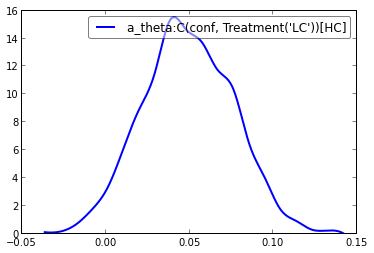
\includegraphics{hddm_demo_fig_08.png}

The above posterior shows that the effect of trial to trial variations
in frontal theta are to increase the estimated decision threshold: the
regression coefficient is positive, and more than 96\% of it is greater
than zero.

As noted above, this experiment also tested patients on deep brain
stimulation (dbs). The full model in the paper thus allowed an
additional factor to estimate how dbs interacts with theta-threshold
relationship. Here we show for illustrative purposes that we can capture
the same effect by simply fitting a separate model to data only
including the case when dbs was turned on. You should see below that in
this case, the influence of theta on threshold reverses. This exercise
thus shows that HDDM can be used both to assess the influence of
trial-by-trial brain measures on DDM parameters, but also how parameters
vary when brain state is manipulated.
\DUspan{name}{}\DUspan{operator}{}\DUspan{name}{}\DUspan{operator}{}\DUspan{name}{}\DUspan{punctuation}{}\DUspan{name}{}\DUspan{punctuation}{}\DUspan{name}{}\DUspan{operator}{}\DUspan{name}{}\DUspan{operator}{}\DUspan{literal,number,integer}{}\DUspan{punctuation}{}\DUspan{literal,string}{}\DUspan{punctuation}{}\DUspan{name}{}\DUspan{operator}{}\DUspan{punctuation}{}\DUspan{literal,string}{}\DUspan{punctuation}{}\DUspan{literal,string}{}\DUspan{punctuation}{}\DUspan{name}{}\DUspan{operator}{}\DUspan{name,builtin,pseudo}{}\DUspan{punctuation}{}
\begin{Verbatim}[commandchars=\\\{\}]
\PYG{n}{m\PYGZus{}reg\PYGZus{}off} \PYG{o}{=} \PYG{n}{hddm}\PYG{o}{.}\PYG{n}{HDDMRegressor}\PYG{p}{(}\PYG{n}{data}\PYG{p}{[}\PYG{n}{data}\PYG{o}{.}\PYG{n}{dbs} \PYG{o}{==} \PYG{l+m+mi}{1}\PYG{p}{]}\PYG{p}{,}
                               \PYG{l+s}{\PYGZdq{}}\PYG{l+s}{a \PYGZti{} theta:C(conf, Treatment(}\PYG{l+s}{\PYGZsq{}}\PYG{l+s}{LC}\PYG{l+s}{\PYGZsq{}}\PYG{l+s}{))}\PYG{l+s}{\PYGZdq{}}\PYG{p}{,}
                               \PYG{n}{depends\PYGZus{}on}\PYG{o}{=}\PYG{p}{\PYGZob{}}\PYG{l+s}{\PYGZsq{}}\PYG{l+s}{v}\PYG{l+s}{\PYGZsq{}}\PYG{p}{:} \PYG{l+s}{\PYGZsq{}}\PYG{l+s}{stim}\PYG{l+s}{\PYGZsq{}}\PYG{p}{\PYGZcb{}}\PYG{p}{,}
                               \PYG{n}{group\PYGZus{}only\PYGZus{}regressors}\PYG{o}{=}\PYG{n+nb+bp}{True}\PYG{p}{)}
\end{Verbatim}

\begin{Verbatim}[commandchars=\\\{\}]
Adding these covariates:
['a\_Intercept', "a\_theta:C(conf, Treatment('LC'))[HC]", "a\_theta:C(conf, Treatment('LC'))[LC]"]
\end{Verbatim}
\DUspan{name}{}\DUspan{operator}{}\DUspan{name}{}\DUspan{punctuation}{}\DUspan{literal,number,integer}{}\DUspan{punctuation}{}\DUspan{name}{}\DUspan{operator}{}\DUspan{literal,number,integer}{}\DUspan{punctuation}{}
\begin{Verbatim}[commandchars=\\\{\}]
\PYG{n}{m\PYGZus{}reg\PYGZus{}off}\PYG{o}{.}\PYG{n}{sample}\PYG{p}{(}\PYG{l+m+mi}{5000}\PYG{p}{,} \PYG{n}{burn}\PYG{o}{=}\PYG{l+m+mi}{200}\PYG{p}{)}
\end{Verbatim}
\DUspan{name}{}\DUspan{operator}{}\DUspan{name}{}\DUspan{operator}{}\DUspan{name}{}\DUspan{operator}{}\DUspan{name}{}\DUspan{punctuation}{}\DUspan{literal,string}{}\DUspan{punctuation}{}\DUspan{name}{}\DUspan{operator}{}\DUspan{name}{}\DUspan{operator}{}\DUspan{name}{}\DUspan{punctuation}{}\DUspan{name}{}\DUspan{punctuation}{}\DUspan{name}{}\DUspan{operator}{}\DUspan{literal,number,integer}{}\DUspan{punctuation}{}\DUspan{keyword}{}\DUspan{literal,string}{}\DUspan{punctuation}{}\DUspan{punctuation}{}\DUspan{name}{}\DUspan{operator}{}\DUspan{name}{}\DUspan{punctuation}{}\DUspan{operator}{}\DUspan{literal,number,integer}{}\DUspan{punctuation}{}\DUspan{operator}{}\DUspan{name}{}\DUspan{punctuation}{}
\begin{Verbatim}[commandchars=\\\{\}]
\PYG{n}{theta} \PYG{o}{=} \PYG{n}{m\PYGZus{}reg\PYGZus{}off}\PYG{o}{.}\PYG{n}{nodes\PYGZus{}db}\PYG{o}{.}\PYG{n}{node}\PYG{p}{[}\PYG{l+s}{\PYGZdq{}}\PYG{l+s}{a\PYGZus{}theta:C(conf, Treatment(}\PYG{l+s}{\PYGZsq{}}\PYG{l+s}{LC}\PYG{l+s}{\PYGZsq{}}\PYG{l+s}{))[HC]}\PYG{l+s}{\PYGZdq{}}\PYG{p}{]}
\PYG{n}{kabuki}\PYG{o}{.}\PYG{n}{analyze}\PYG{o}{.}\PYG{n}{plot\PYGZus{}posterior\PYGZus{}nodes}\PYG{p}{(}\PYG{p}{[}\PYG{n}{theta}\PYG{p}{]}\PYG{p}{,} \PYG{n}{bins}\PYG{o}{=}\PYG{l+m+mi}{10}\PYG{p}{)}
\PYG{k}{print} \PYG{l+s}{\PYGZdq{}}\PYG{l+s}{P(a\PYGZus{}theta \PYGZgt{} 0) = }\PYG{l+s}{\PYGZdq{}}\PYG{p}{,} \PYG{p}{(}\PYG{n}{theta}\PYG{o}{.}\PYG{n}{trace}\PYG{p}{(}\PYG{p}{)} \PYG{o}{\PYGZgt{}} \PYG{l+m+mi}{0}\PYG{p}{)}\PYG{o}{.}\PYG{n}{mean}\PYG{p}{(}\PYG{p}{)}
\end{Verbatim}

\begin{Verbatim}[commandchars=\\\{\}]
\PYG{n}{P}\PYG{p}{(}\PYG{n}{a\PYGZus{}theta} \PYG{o}{\PYGZgt{}} \PYG{l+m+mi}{0}\PYG{p}{)} \PYG{o}{=}  \PYG{l+m+mf}{0.0122916666667}
\end{Verbatim}

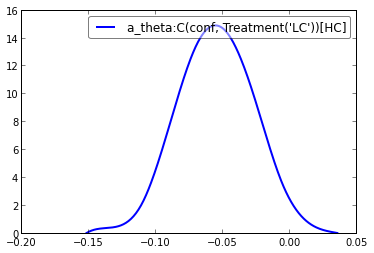
\includegraphics{hddm_demo_fig_09.png}


\subsection{Dealing with outliers}
\label{demo:dealing-with-outliers}
It is common to have outliers in any data set and RT data is no
exception. Outliers present a serious challenge to likelihood-based
approaches, as used in HDDM. Consider the possibility that 5\% of trials
are not generated by the DDM process, but by some other process (e.g.
due to an attentional lapse). The observed data in those trials may be
very unlikely given the best DDM parameters that fit 95\% of the data. In
the extreme case, the likelihood of a single trial may be zero (e.g. if
subjects respond very quickly, faster than the non-decision time \code{t}
parameter that would fit the rest of the data). Thus this single outlier
would force the DDM parameters to adjust substantially. To see the
effect of this we will generate data with outliers, but fit a standard
DDM model without taking outliers into account.
\DUspan{name}{}\DUspan{punctuation}{}\DUspan{name}{}\DUspan{operator}{}\DUspan{name}{}\DUspan{operator}{}\DUspan{name}{}\DUspan{operator}{}\DUspan{name}{}\DUspan{punctuation}{}\DUspan{name}{}\DUspan{operator}{}\DUspan{punctuation}{}\DUspan{literal,string}{}\DUspan{punctuation}{}\DUspan{literal,number,integer}{}\DUspan{punctuation}{}\DUspan{literal,string}{}\DUspan{punctuation}{}\DUspan{operator}{}\DUspan{literal,number,integer}{}\DUspan{punctuation}{}\DUspan{literal,string}{}\DUspan{punctuation}{}\DUspan{operator}{}\DUspan{literal,number,integer}{}\DUspan{punctuation}{}\DUspan{name}{}\DUspan{operator}{}\DUspan{literal,number,integer}{}\DUspan{punctuation}{}\DUspan{name}{}\DUspan{operator}{}\DUspan{literal,number,integer}{}\DUspan{punctuation}{}
\begin{Verbatim}[commandchars=\\\{\}]
\PYG{n}{outlier\PYGZus{}data}\PYG{p}{,} \PYG{n}{params} \PYG{o}{=} \PYG{n}{hddm}\PYG{o}{.}\PYG{n}{generate}\PYG{o}{.}\PYG{n}{gen\PYGZus{}rand\PYGZus{}data}\PYG{p}{(}\PYG{n}{params}\PYG{o}{=}\PYG{p}{\PYGZob{}}\PYG{l+s}{\PYGZsq{}}\PYG{l+s}{a}\PYG{l+s}{\PYGZsq{}}\PYG{p}{:} \PYG{l+m+mi}{2}\PYG{p}{,} \PYG{l+s}{\PYGZsq{}}\PYG{l+s}{t}\PYG{l+s}{\PYGZsq{}}\PYG{p}{:} \PYG{o}{.}\PYG{l+m+mi}{4}\PYG{p}{,} \PYG{l+s}{\PYGZsq{}}\PYG{l+s}{v}\PYG{l+s}{\PYGZsq{}}\PYG{p}{:} \PYG{o}{.}\PYG{l+m+mi}{5}\PYG{p}{\PYGZcb{}}\PYG{p}{,}
                                                   \PYG{n}{size}\PYG{o}{=}\PYG{l+m+mi}{200}\PYG{p}{,} \PYG{n}{n\PYGZus{}fast\PYGZus{}outliers}\PYG{o}{=}\PYG{l+m+mi}{10}\PYG{p}{)}
\end{Verbatim}
\DUspan{name}{}\DUspan{operator}{}\DUspan{name}{}\DUspan{operator}{}\DUspan{name}{}\DUspan{punctuation}{}\DUspan{name}{}\DUspan{punctuation}{}\DUspan{name}{}\DUspan{operator}{}\DUspan{name}{}\DUspan{punctuation}{}\DUspan{literal,number,integer}{}\DUspan{punctuation}{}\DUspan{name}{}\DUspan{operator}{}\DUspan{literal,number,integer}{}\DUspan{punctuation}{}
\begin{Verbatim}[commandchars=\\\{\}]
\PYG{n}{m\PYGZus{}no\PYGZus{}outlier} \PYG{o}{=} \PYG{n}{hddm}\PYG{o}{.}\PYG{n}{HDDM}\PYG{p}{(}\PYG{n}{outlier\PYGZus{}data}\PYG{p}{)}
\PYG{n}{m\PYGZus{}no\PYGZus{}outlier}\PYG{o}{.}\PYG{n}{sample}\PYG{p}{(}\PYG{l+m+mi}{2000}\PYG{p}{,} \PYG{n}{burn}\PYG{o}{=}\PYG{l+m+mi}{50}\PYG{p}{)}
\end{Verbatim}
\DUspan{name}{}\DUspan{operator}{}\DUspan{name}{}\DUspan{punctuation}{}
\begin{Verbatim}[commandchars=\\\{\}]
\PYG{n}{m\PYGZus{}no\PYGZus{}outlier}\PYG{o}{.}\PYG{n}{plot\PYGZus{}posterior\PYGZus{}predictive}\PYG{p}{(}\PYG{p}{)}
\end{Verbatim}

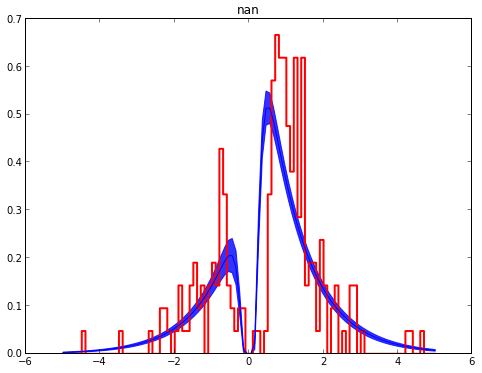
\includegraphics{hddm_demo_fig_10.png}

As you can see, the predictive likelihood does not fit the RT data very
well. The model predicts far more RTs near the leading edge of the
distribution than are actually observed. This is because non-decision
time \code{t} is forced to be estimated small enough to account for a few
fast RTs.

What we can do instead is fit a mixture model which assumes that
outliers come from a uniform distribution. (Note, outliers do not have
to be very fast or very slow, and the above example is just an obvious
illustration. Some proportion of the trials can be assumed to simply
come from a different process for which we make no assumptions about its
generation, and hence use a uniform distribution. This allows the model
to find the best DDM parameters that capture the majority of trials).
Here, we specify that we expect roughly 5\% outliers in our data.
\DUspan{name}{}\DUspan{operator}{}\DUspan{name}{}\DUspan{operator}{}\DUspan{name}{}\DUspan{punctuation}{}\DUspan{name}{}\DUspan{punctuation}{}\DUspan{name}{}\DUspan{operator}{}\DUspan{literal,number,oct}{}\DUspan{punctuation}{}\DUspan{name}{}\DUspan{operator}{}\DUspan{name}{}\DUspan{punctuation}{}\DUspan{literal,number,integer}{}\DUspan{punctuation}{}\DUspan{name}{}\DUspan{operator}{}\DUspan{literal,number,integer}{}\DUspan{punctuation}{}
\begin{Verbatim}[commandchars=\\\{\}]
\PYG{n}{m\PYGZus{}outlier} \PYG{o}{=} \PYG{n}{hddm}\PYG{o}{.}\PYG{n}{HDDM}\PYG{p}{(}\PYG{n}{outlier\PYGZus{}data}\PYG{p}{,} \PYG{n}{p\PYGZus{}outlier}\PYG{o}{=}\PYG{o}{.}\PYG{l+m+mo}{05}\PYG{p}{)}
\PYG{n}{m\PYGZus{}outlier}\PYG{o}{.}\PYG{n}{sample}\PYG{p}{(}\PYG{l+m+mi}{2000}\PYG{p}{,} \PYG{n}{burn}\PYG{o}{=}\PYG{l+m+mi}{20}\PYG{p}{)}
\end{Verbatim}
\DUspan{name}{}\DUspan{operator}{}\DUspan{name}{}\DUspan{punctuation}{}
\begin{Verbatim}[commandchars=\\\{\}]
\PYG{n}{m\PYGZus{}outlier}\PYG{o}{.}\PYG{n}{plot\PYGZus{}posterior\PYGZus{}predictive}\PYG{p}{(}\PYG{p}{)}
\end{Verbatim}

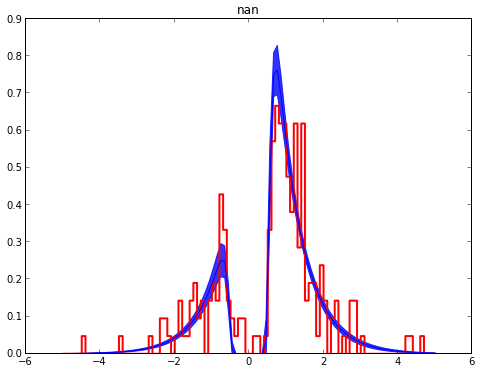
\includegraphics{hddm_demo_fig_11.png}

As you can see, the model provides a much better fit. The outlier RTs
are having less of an effect because they get assigned to the uniform
outlier distribution.

\section{Discussion}
We developed an open-source Python toolbox that allows hierarchical Bayesian parameter estimation of the DDM and LBA and is successfully being used in various experimental psychology and neurocognitive research laboratories. The DDM and LBA can be used to infer latent psychological processes underlying decision making given reaction time and choice data. Since its first release in 2011, HDDM has been downloaded over 8000 times on PyPI and attracted an active community of users that frequently interact on the \href{https://groups.google.com/group/hddm-users/}{HDDM-users mailing   list}. The benefit of the hierarchical Bayesian approach is two-fold: (i) improved accuracy of individual subject parameter recover by modeling subject similarity in a hierarchical fashion; and (ii) full Bayesian posterior inference that obsoletes frequentist statistics and confidence intervals. Despite prior methodological advancements in this area, a reliable software package implementing this method was previously not available. Special care has been taken to make this software easy to install and use. A simple yet powerful model description mechanism allows the creation of arbitrarily complex models where separate parameters can be estimated for different conditions. Additional features like posterior-predictive-checks allow for model validation and comparison. Finally, to facilitate cross-domain application of this toolbox in the cognitive neurosciences, it is simple to estimate trial-by-trial influences of e.g. brain-measures on individual model parameters.

\section{Acknowledgements}
The software was written by TVW and IS. The paper was written by TVW and MJF. The authors are thankful to Guido Biele and Øystein Sandvik for useful feedback and code contributions.

\bibliographystyle{plainnat}
\bibliography{hddm}


\renewcommand{\indexname}{Index}
\printindex
\end{document}
